% Options for packages loaded elsewhere
\PassOptionsToPackage{unicode}{hyperref}
\PassOptionsToPackage{hyphens}{url}
\documentclass[
  10pt,
  ignorenonframetext,
  aspectratio=43,
  english,
  handout]{beamer}
\newif\ifbibliography
\usepackage{pgfpages}
\setbeamertemplate{caption}[numbered]
\setbeamertemplate{caption label separator}{: }
\setbeamercolor{caption name}{fg=normal text.fg}
\beamertemplatenavigationsymbolsempty
% remove section numbering
\setbeamertemplate{part page}{
  \centering
  \begin{beamercolorbox}[sep=16pt,center]{part title}
    \usebeamerfont{part title}\insertpart\par
  \end{beamercolorbox}
}
\setbeamertemplate{section page}{
  \centering
  \begin{beamercolorbox}[sep=12pt,center]{section title}
    \usebeamerfont{section title}\insertsection\par
  \end{beamercolorbox}
}
\setbeamertemplate{subsection page}{
  \centering
  \begin{beamercolorbox}[sep=8pt,center]{subsection title}
    \usebeamerfont{subsection title}\insertsubsection\par
  \end{beamercolorbox}
}
% Prevent slide breaks in the middle of a paragraph
\widowpenalties 1 10000
\raggedbottom
\AtBeginPart{
  \frame{\partpage}
}
\AtBeginSection{
  \ifbibliography
  \else
    \frame{\sectionpage}
  \fi
}
\AtBeginSubsection{
  \frame{\subsectionpage}
}
\usepackage{iftex}
\ifPDFTeX
  \usepackage[T1]{fontenc}
  \usepackage[utf8]{inputenc}
  \usepackage{textcomp} % provide euro and other symbols
\else % if luatex or xetex
  \usepackage{unicode-math} % this also loads fontspec
  \defaultfontfeatures{Scale=MatchLowercase}
  \defaultfontfeatures[\rmfamily]{Ligatures=TeX,Scale=1}
\fi
\usepackage{lmodern}
\usetheme[progressbar=frametitle,block=fill,subsectionpage=progressbar]{metropolis}
\ifPDFTeX\else
  % xetex/luatex font selection
\fi
% Use upquote if available, for straight quotes in verbatim environments
\IfFileExists{upquote.sty}{\usepackage{upquote}}{}
\IfFileExists{microtype.sty}{% use microtype if available
  \usepackage[]{microtype}
  \UseMicrotypeSet[protrusion]{basicmath} % disable protrusion for tt fonts
}{}
\makeatletter
\@ifundefined{KOMAClassName}{% if non-KOMA class
  \IfFileExists{parskip.sty}{%
    \usepackage{parskip}
  }{% else
    \setlength{\parindent}{0pt}
    \setlength{\parskip}{6pt plus 2pt minus 1pt}}
}{% if KOMA class
  \KOMAoptions{parskip=half}}
\makeatother
\ifLuaTeX
\usepackage[bidi=basic,shorthands=off]{babel}
\else
\usepackage[bidi=default,shorthands=off]{babel}
\fi
\ifLuaTeX
  \usepackage{selnolig} % disable illegal ligatures
\fi
\setlength{\emergencystretch}{3em} % prevent overfull lines
\providecommand{\tightlist}{%
  \setlength{\itemsep}{0pt}\setlength{\parskip}{0pt}}
% preamble carried over from the LyX source
\usepackage{tikz}
\usetikzlibrary{positioning}
\usetikzlibrary{overlay-beamer-styles}
\usepackage{appendixnumberbeamer}

\usepackage{graphicx}
\usepackage{subfig}


% margin
\setbeamersize{text margin right=1.5cm}

% colors
\colorlet{DarkRed}{red!70!black}
\setbeamercolor{normal text}{fg=black}
\setbeamercolor{alerted text}{fg=DarkRed}
\setbeamercolor{progress bar}{fg=DarkRed}
\setbeamercolor{button}{bg=DarkRed}

% width of seperators
\makeatletter
\setlength{\metropolis@titleseparator@linewidth}{1pt}
\setlength{\metropolis@progressonsectionpage@linewidth}{1pt}
\setlength{\metropolis@progressinheadfoot@linewidth}{1pt}
\makeatother

% new alert block
\newlength\origleftmargini
\setlength\origleftmargini\leftmargini
\setbeamertemplate{itemize/enumerate body begin}{\setlength{\leftmargini}{4mm}}
\let\oldalertblock\alertblock
\let\oldendalertblock\endalertblock
\def\alertblock{\begingroup \setbeamertemplate{itemize/enumerate body begin}{\setlength{\leftmargini}{\origleftmargini}} \oldalertblock}
\def\endalertblock{\oldendalertblock \endgroup}
\setbeamertemplate{mini frame}{}
\setbeamertemplate{mini frame in current section}{}
\setbeamertemplate{mini frame in current subsection}{}
\setbeamercolor{section in head/foot}{fg=normal text.bg, bg=structure.fg}
\setbeamercolor{subsection in head/foot}{fg=normal text.bg, bg=structure.fg}

% footer
\makeatletter
\setbeamertemplate{footline}{%
    \begin{beamercolorbox}[colsep=1.5pt]{upper separation line head}
    \end{beamercolorbox}
    \begin{beamercolorbox}{section in head/foot}
      \vskip1pt\insertsectionnavigationhorizontal{\paperwidth}{}{\hskip0pt plus1filll \insertframenumber{} / \inserttotalframenumber \hskip2pt}\vskip3pt%
    \end{beamercolorbox}%
    \begin{beamercolorbox}[colsep=1.5pt]{lower separation line head}
    \end{beamercolorbox}
}
\makeatother

% toc
\setbeamertemplate{section in toc}{\hspace*{1em}\inserttocsectionnumber.~\inserttocsection\par}
\setbeamertemplate{subsection in toc}{\hspace*{2em}\inserttocsectionnumber.\inserttocsubsectionnumber.~\inserttocsubsection\par}

% code
\usepackage{xcolor}
\usepackage{listings}

\definecolor{codegray}{rgb}{0.5,0.5,0.5}
\definecolor{background}{HTML}{F5F5F5}
\definecolor{keyword}{HTML}{4B69C6}
\definecolor{string}{HTML}{448C27}
\definecolor{comment}{HTML}{448C27}

\usepackage{inconsolata}
\lstdefinestyle{mystyle}{
    commentstyle=\color{comment},
    keywordstyle=\color{keyword},
    stringstyle=\color{string},
    basicstyle=\ttfamily,
    breakatwhitespace=false,
    breaklines=true,
    captionpos=b,
    keepspaces=true,
    numbersep=5pt,
    showspaces=false,
    showstringspaces=false,
    showtabs=false,
    tabsize=4,
	showlines=true
}

\lstset{style=mystyle}
% Added by lyx2lyx
\setlength{\parskip}{\smallskipamount}
\setlength{\parindent}{0pt}

\usepackage{bookmark}
\IfFileExists{xurl.sty}{\usepackage{xurl}}{} % add URL line breaks if available
\urlstyle{same}
\hypersetup{
  pdftitle={Consumption-Saving},
  pdfauthor={Raphaël Huleux},
  pdflang={en},
  hidelinks,
  pdfcreator={LaTeX via pandoc}}

\title{\texorpdfstring{Consumption-Saving}{Consumption-Saving}}
\subtitle{\texorpdfstring{Adv. Macro: Heterogeneous Agent
Models}{Adv. Macro: Heterogeneous Agent Models}}
\author{\texorpdfstring{Raphaël Huleux}{Raphaël Huleux}}
\date{2026}

\begin{document}
\frame{\titlepage}

\section{Introduction}\label{introduction}

\begin{frame}{\alt<2>{We open the household block}{A model is a set of blocks}}
\protect\phantomsection\label{section}
\vspace{2mm}

\begin{center}
\begin{tikzpicture}[
block/.style={draw,thick,rounded corners,minimum width=3.1cm,minimum height=1cm,align=center},
lbl/.style={font=\scriptsize,alt=<2>{text=black!20}{}},
dim/.style={alt=<2>{draw=black!20,text=black!20}{}},
hl/.style={alt=<2>{draw=DarkRed,very thick,fill=DarkRed!10,text=DarkRed}{}}]

\node[block,dim] (gov) at (3.4,1.85) {Government};
\node[block,hl] (hh) at (0,0) {Households};
\node[block,dim] (firm) at (6.8,0) {Firms};
\node[block,dim] (mkt) at (3.4,-1.85) {Market clearing};

\draw[->,thick,dim] (hh.north east) -- node[lbl,above,sloped]{$N_{t}$, $A_{t}$} (firm.north west);
\draw[->,thick,dim] (firm.south west) -- node[lbl,below,sloped]{$r_{t}$, $w_{t}$} (hh.south east);
\draw[->,thick,dim] (gov.west) -- node[lbl,above,sloped]{$\tau_{t}$, transfers} (hh.north);
\draw[->,thick,dim] (gov.east) -- node[lbl,above,sloped]{$B_{t}$, $G_{t}$} (firm.north);
\draw[->,thick,dim] (hh.south) -- node[lbl,below,sloped]{$C_{t}$, $A_{t}$} (mkt.west);
\draw[->,thick,dim] (firm.south) -- node[lbl,below,sloped]{$Y_{t}$, $K_{t}$} (mkt.east);

\end{tikzpicture}
\end{center}

\vspace{1mm}

\begin{overlayarea}{\textwidth}{1.85cm}
\only<1|handout:0>{\textbf{Every block is a set of equations }mapping inputs into outputs.}
\only<2>{%
\textbf{This course focuses on the household block.}

\vspace{2mm}
\textbf{The question: }\emph{when does the distribution matter for aggregates?}%
}
\end{overlayarea}
\end{frame}

\begin{frame}{Goals for today}
\protect\phantomsection\label{goals-for-today}
\begin{itemize}
\tightlist
\item
  \textbf{Review consumption-saving theory}

  \begin{enumerate}
  \tightlist
  \item
    The permanent income hypothesis, and what it gets wrong
  \item
    The buffer-stock model: risk and borrowing constraints
  \end{enumerate}
\item
  \textbf{Solve the household problem in partial equilibrium}

  \begin{enumerate}
  \tightlist
  \item
    Basics of dynamic programming
  \item
    Value function iteration (VFI)
  \item
    The endogenous grid method (EGM)
  \end{enumerate}
\item
  \textbf{Simulate the distribution and aggregate}

  \begin{enumerate}
  \tightlist
  \item
    Monte Carlo
  \item
    The histogram method (Young, 2010)
  \end{enumerate}
\item
  \textbf{Note:} partial equilibrium for now, prices are \emph{fixed}.
  They become equilibrium objects in the next lecture.
\end{itemize}
\end{frame}

\begin{frame}{Literature}
\protect\phantomsection\label{literature}
\begin{itemize}
\tightlist
\item
  \textbf{Generations of models:}

  \begin{enumerate}
  \tightlist
  \item
    \textbf{Permanent income hypothesis (PIH)} (Friedman, 1957)\\
    or life-cycle model (Modigliani and Brumberg, 1954)
  \item
    \textbf{Buffer-stock consumption model}\\
    Deaton (1991, 1992); Carroll (1992, 1997, 2019)
  \item
    \textbf{Multiple-asset buffer-stock consumption models}\\
    e.g.~Kaplan and Violante (2014); Harmenberg and Öberg (2021)
  \end{enumerate}
\item
  \textbf{Consumption-and-saving over the life-cycle dynamic}\\
  e.g.~Gourinchas and Parker (2002); Druedahl and Martinello (2022)
\item
  \textbf{Empirical MPCs and income risk}\\
  e.g.~Fagereng et al.~(2021); Guvenen et al.~(2021)
\end{itemize}

\textbf{Book:}
\href{https://global.oup.com/academic/product/the-economics-of-consumption-9780199383153?cc=dk&lang=en&}{The
Economics of Consumption}, Jappelli and Pistaferri (2017)
\end{frame}

\begin{frame}{Plan}
\protect\phantomsection\label{plan}
\tableofcontents[]
\end{frame}

\section{PIH}\label{pih}

\begin{frame}{Keynes vs Friedman}
\protect\phantomsection\label{keynes-vs-friedman}
\begin{itemize}
\tightlist
\item
  \textbf{Keynesian consumption function:} \(C_{t}=\bar{C}+bY_{t}\)
  Consumption responds to \emph{current} income. Multiplier is
  \(\frac{1}{1-b}\).\\
  But it lacks micro-foundations!
\item
  \textbf{Permanent income hypothesis} (Friedman, 1957)\textbf{:}
  Consumption responds to the \emph{present value} of income.\\
  Current income matters only through it.
\item
  But: PIH implies too low MPCs. We will see how to fix it
\end{itemize}
\end{frame}

\begin{frame}{Consumption-saving}
\protect\phantomsection\label{consumption-saving}
\[
\begin{aligned}
v_{0} & =\max_{\{c_{t}\}^{T-1}_{t=0}}\sum^{T-1}_{t=0}\beta^{t}u(c_{t})\\
& \text{s.t.}\\
a_{t} & =(1+r)a_{t-1}+wz_{t}-c_{t}\\
a_{T-1} & \geq0, \quad a_{-1}\  \text{given}
\end{aligned}
\]

\begin{itemize}
\item
  \textbf{Variables:} Consumption: \(c_{t}\) Productivity: \(z_{t}\)
  End-of-period savings: \(a_{t}\) (\emph{no debt at death})
\item
  \textbf{Parameters:} Discount factor: \(\beta\) Wage: \(w\) Interest
  rate: \(r\) (define \(R\equiv1+r\) as interest factor)
\end{itemize}
\end{frame}

\begin{frame}{IBC}
\protect\phantomsection\label{ibc}
\begin{itemize}
\tightlist
\item
  \textbf{Only the terminal condition really constrains:} without
  \(a_{T-1}\geq0\) the household would just borrow more and more
\item
  \textbf{Substitution} implies \emph{Intertemporal Budget Constraint}
  (IBC) \[
    \begin{aligned}
    a_{T-1} & = & Ra_{T-2}+wz_{T-1}-c_{T-1}\\
    & = & R(Ra_{T-3}+wz_{T-2}-c_{T-2})+wz_{T-1}-c_{T-1}\\
    & = & R^{T}a_{-1}+\sum^{T-1}_{t=0}R^{T-1-t}(wz_{t}-c_{t})
    \end{aligned}
    \]
\item
  Use \textbf{terminal condition} \(a_{T-1}=0\) (equality due to utility
  max.) \[
    \begin{aligned}
    R^{-(T-1)}a_{T-1}=0 & \Leftrightarrow & \sum^{T-1}_{t=0}R^{-t}c_{t}=s_{0}+h_{0}
    \end{aligned}
    \] where \(s_{0}\equiv Ra_{-1}\) (after-interest assets) and
  \(h_{0}\equiv\sum^{T-1}_{t=0}R^{-t}wz_{t}\) (human capital)
\end{itemize}
\end{frame}

\begin{frame}{FOC and Euler-equation}
\protect\phantomsection\label{foc-and-euler-equation}
\[
\mathcal{L}=\sum^{T-1}_{t=0}\beta^{t}u(c_{t})+\lambda\left[s_{0}+h_{0}-\sum^{T-1}_{t=0}R^{-t}c_{t}\right]
\] - \textbf{It is a \emph{static} problem:} 1. \textbf{Information:}
\(s_{0}\) and \(h_{0}\) are known at \(t=0\) 2. \textbf{Target:}
Discounted utility, \(\sum^{T-1}_{t=0}\beta^{t}u(c_{t})\) 3.
\textbf{Behavior:} Choose \(c_{0},c_{1},\dots,c_{T-1}\)
\emph{simultaneously} 4. \textbf{Solution:} Sequence of consumption
\emph{choices} \(c^{\ast}_{0},c^{\ast}_{1},\dots,c^{\ast}_{T-1}\) -
\textbf{First order conditions}: \[
    \forall t:0=\beta^{t}u^{\prime}(c_{t})-\lambda R^{-t}\Leftrightarrow u^{\prime}(c_{t})=\lambda\left(\beta R\right)^{-t}
    \] - \textbf{Euler-equation} for \(k\in\{1,2,\dots\}\): \[
    \frac{u^{\prime}(c_{t})}{u^{\prime}(c_{t+k})}=\frac{\lambda\left(\beta R\right)^{-t}}{\lambda\left(\beta R\right)^{-(t+k)}}=\left(\beta R\right)^{k}
    \]
\end{frame}

\begin{frame}{Consumption choice}
\protect\phantomsection\label{consumption-choice}
\begin{itemize}
\tightlist
\item
  \textbf{CRRA:} \(u(c_{t})=\frac{c^{1-\sigma}_{t}}{1-\sigma}\) implies
  the Euler-equation \[
    \frac{c^{-\sigma}_{0}}{c^{-\sigma}_{t}}=\left(\beta R\right)^{t}\Leftrightarrow c_{t}=(\beta R)^{\frac{t}{\sigma}}c_{0}
    \] Constant consumption if:

  \begin{enumerate}
  \tightlist
  \item
    \(\beta R=1\)
  \item
    \(\frac{1}{\sigma}\rightarrow0\) (zero intertemporal elasticity of
    substitution)
  \end{enumerate}
\item
  Insert \textbf{Euler} into \textbf{IBC} to get consumption choice \[
    \begin{aligned}
    \sum^{T-1}_{t=0}\left((\beta R)^{1/\sigma}R^{-1}\right)^{t}c_{0} & = && (s_{0}+h_{0})\Leftrightarrow\\
    c^{\ast}_{0} & =  \frac{1-(\beta R)^{1/\sigma}R^{-1}}{1-\left((\beta R)^{1/\sigma}R^{-1}\right)^{T}}&&(s_{0}+h_{0})
    \end{aligned}
    \]
\end{itemize}
\end{frame}

\begin{frame}{Infinite horizon: \(T\rightarrow\infty\)}
\protect\phantomsection\label{infinite-horizon-trightarrowinfty}
\begin{itemize}
\tightlist
\item
  \textbf{Infinite horizon} for \((\beta R)^{1/\sigma}R^{-1}<1\): Let
  \(T\rightarrow\infty\) to get \[
    \begin{aligned}
    c^{\ast}_{0} & =\left(1-\frac{(\beta R)^{1/\sigma}}{R}\right)(s_{0}+h_{0})
    \end{aligned}
    \] Assuming \(\beta R =1\), this becomes
  \[c_{0} = \frac{r}{1+r}(s_{0}+h_{0}) \] \(\Rightarrow\) Consumption is
  the annuity value of total wealth (perfect consumption smoothing!)
\end{itemize}
\end{frame}

\begin{frame}[fragile]{Consumption smoothing}
\protect\phantomsection\label{consumption-smoothing}
\begin{center}
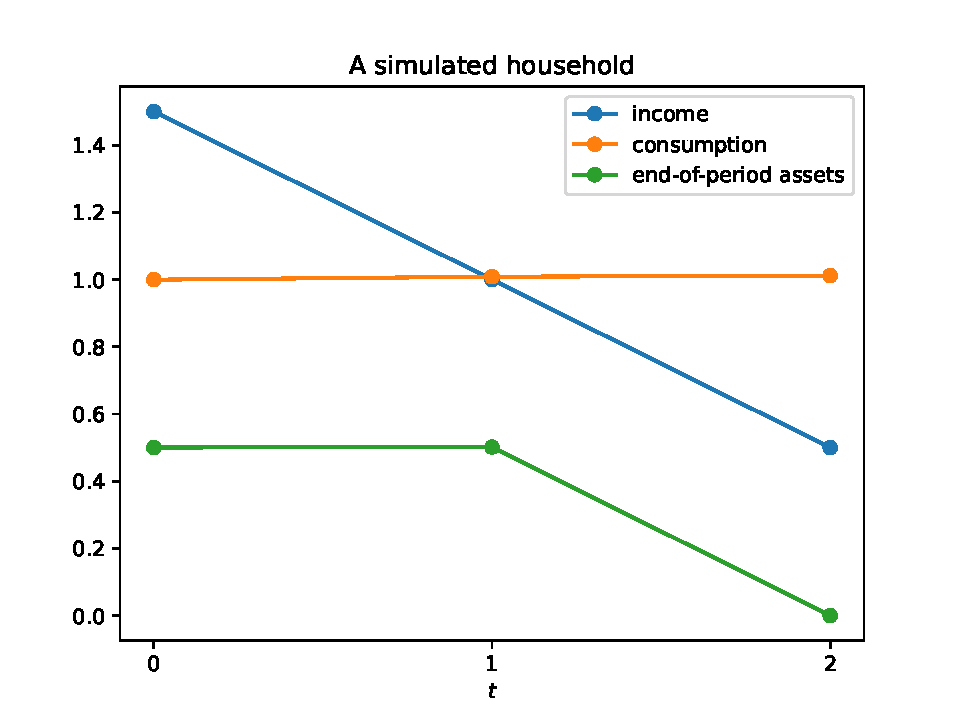
\includegraphics[width=0.72\textwidth]{figs/pih_simulation}
\end{center}

\textbf{Income falls by two thirds, consumption stays almost constant.}
The household saves while income is high and runs the savings down when
it is low. (\(T=3\), \(a_{-1}=0\), from
\texttt{02\textbackslash{}\_vfi\textbackslash{}\_pih.ipynb})
\end{frame}

\begin{frame}{Propensities to consume (\(\beta R=1\), \(z_{t}=1\))}
\protect\phantomsection\label{propensities-to-consume-beta-r1-z_t1}
Assume \(\beta R=1\) and \(z_{t}=1\), then \[
c^{\ast}_{0}= ra_{-1}+w
\] \textbf{MPC for different types of shocks} (exact derivatives):

\begin{enumerate}
\tightlist
\item
  MPC of \emph{windfall} income:
  \(\frac{\partial c_{0}}{\partial s_{0}}=\frac{r}{1+r}\approx r\)
\item
  MPC of \emph{future} income change:
  \(\frac{\partial c_{0}}{\partial wz_{t}}=\frac{r}{1+r}\left(1+r\right)^{-t}\)
  \(\to\) even smaller
\item
  MPC of \emph{permanent} income change:
  \(\frac{\partial c_{0}}{\partial w}=1\)
\end{enumerate}
\end{frame}

\begin{frame}{Connection to the representative agent}
\protect\phantomsection\label{connection-to-the-representative-agent}
\begin{itemize}
\item
  \textbf{The consumption function is} \emph{linear} \textbf{in
  resources} \[
    c^{\ast}_{0}=\kappa\left(s_{0}+h_{0}\right),\qquad\kappa\equiv1-\frac{(\beta R)^{1/\sigma}}{R}
    \] with the \emph{same} \(\kappa\) for every household
\item
  \textbf{Exact aggregation:} sum over households \(i\)
  \[ \sum_{i}c^{\ast}_{0,i}=\kappa\left(\sum_{i}s_{0,i}+\sum_{i}h_{0,i}\right)
    \]
\item
  \textbf{Implication:} aggregate consumption depends on
  \emph{aggregate} wealth and \emph{aggregate} income only. The
  distribution does not enter, and a representative agent gets the
  aggregates exactly right.
\item
  \textbf{This is why the course exists:} \emph{heterogeneity matters
  for aggregates only once this linearity breaks.}
\end{itemize}
\end{frame}

\section{Dynamic programming}\label{dynamic-programming}

\begin{frame}{Derive the Bellman equation}
\protect\phantomsection\label{derive-the-bellman-equation}
Rewrite the consumption savings problem \[
\begin{aligned}
    v_{t}(a_{t-1}) &= \max_{\{c_{s}\}_{s=t}^{T-1}} \sum_{s=t}^{T-1} \beta^{s-t} u(c_{s}) \\
    &= \max_{\{c_{s}\}_{s=t}^{T-1}} \Big[ u(c_{t}) + \beta \sum_{s=t+1}^{T-1}  \beta^{s-t-1} u(c_{s})\Big] \\
    &= \max_{c_{t}} \Bigg[ u(c_{t}) + \beta \underbrace{\max_{\{c_{s}\}_{s=t+1}^{T-1}}\Big[ \sum_{s=t+1}^{T-1}  \beta^{s-(t+1)} u(c_{s})\Big]}_{=v_{t+1}(a_{t})} \Bigg]  \\
    &= \max_{c_{t}} \Big[ u(c_{t})+\beta v_{t+1}(a_{t})\Big]
\end{aligned}
\]

This is called the \textbf{Bellman equation}.
\end{frame}

\begin{frame}{Dynamic Programming vs Sequence Problem}
\protect\phantomsection\label{dynamic-programming-vs-sequence-problem}
\[
v_{t}(a_{t-1})=\max_{c_{t}} \Big[ u(c_{t})+\beta v_{t+1}(a_{t})\Big]
\] Main differences:

\vspace{5mm}

\begin{enumerate}
\tightlist
\item
  Now we maximize only with respect to \(c_t\), not the entire path!
\item
  We obtain \(c^{\ast}_t(a_{t-1})\), which is called a \textbf{policy
  function}
\item
  \(v_{t+1}(a_t)\) is called a \textbf{value function}.
\end{enumerate}

\vspace{5mm}

Solving the problem amounts to finding those two functions! How can we
do it?
\end{frame}

\begin{frame}{Backward induction}
\protect\phantomsection\label{backward-induction}
To solve the problem in finite horizon, we use \textbf{backward
induction}.\\
Let's start from the end. In the last period, \(t=T-1\), we have \[
v_{T-1}(a_{T-2})=\max_{c_{T-1}} u(c_{T-1}) + \beta v_{T}(a_{T-1})
\] There is no period \(T\), so \(v_{T}(a_{T-1})=0\), and with \(a_{T-1}\geq0\) the household consumes everything, \(c_{T-1}=(1+r)a_{T-2}+wz_{T-1}\). Thus: \[
v_{T-1}(a_{T-2}) = u\big((1+r)a_{T-2}+wz_{T-1}\big)
\] We can then go backward in time, and solve \(v_{T-2}(a_{T-3})\), etc,
until \(v_0(a_{-1})\).
\end{frame}

\begin{frame}{Euler equation and envelope condition}
\protect\phantomsection\label{euler-equation-and-envelope-condition}
For \(t<T-1\), substitute the budget constraint into the objective \[
v_{t}(a_{t-1}) = \max_{a_{t}} \Big[u\big((1+r)a_{t-1}+wz_{t}-a_{t}\big)+\beta v_{t+1}(a_{t})\Big]
\]The first-order condition is \(u'(c_{t}) = \beta v'_{t+1}(a_{t})\). \\
To obtain \(v'_{t+1}\), differentiate with respect to the \emph{state}, \(a_{t-1}\): \[
\begin{aligned}
    v'_{t}(a_{t-1}) &= u'(c_{t}) \left(1+r-\frac{\partial a_{t}}{\partial a_{t-1}} \right) + \beta v'_{t+1}(a_{t}) \frac{\partial a_{t}}{\partial a_{t-1}}  \\
    &= u'(c_{t})(1+r) + \frac{\partial a_{t}}{\partial a_{t-1}} \underbrace{\Big(u'(c_{t}) -\beta v'_{t+1}(a_{t})\Big)}_{=0} = u'(c_{t})(1+r)
\end{aligned}
\] This is the \textbf{envelope theorem}!

Shift one period forward and insert in the FOC:
\(u'(c_{t})=\beta R\,u'(c_{t+1})\). Same Euler-equation as in the
sequence problem, hence same solution!
\end{frame}

\begin{frame}{A dynamic programming ``recipe''}
\protect\phantomsection\label{a-dynamic-programming-recipe}
Start at \(t=T-1\) with \(v_{T}(\bullet)=0\). For every possible
\(a_{t-1}\):

\begin{enumerate}
\tightlist
\item Maximize \(u(c_t)+ \beta v_{t+1}(a_{t})\) to get \(c_t^{\ast}(a_{t-1})\)
\item Compute \(v_t(a_{t-1})=u(c_{t}^{\ast}(a_{t-1}))+\beta v_{t+1}(a_{t}^{\ast})\)
\end{enumerate}

Go backward in time, until \(t=0\).

We have obtained a sequence of policy functions \(c_t^{\ast}(a_{t-1})\) and value functions \(v_t(a_{t-1})\)!
\end{frame}

\begin{frame}{We need three computational tools}
\protect\phantomsection\label{we-need-three-computational-tools}
To do this on a computer, we need a couple of things: \vspace{5mm}

\begin{enumerate}
\tightlist
\item How do we loop over all possible \(a_{t-1}\)? $\to$ \textbf{Create a grid}
\item We don't have an analytical expression for \(v_{t+1}(a_t)\). How do we approximate it? $\to$ \textbf{Use linear interpolation}
\item How do we maximize a function? $\to$ \textbf{grid search or golden section search!}
\end{enumerate}
\end{frame}

\begin{frame}{}
\protect\phantomsection\label{section-1}
\begin{center}
\LARGE Let's code!
\end{center}
\end{frame}

\begin{frame}{Infinite Horizon: Convergence}
\protect\phantomsection\label{infinite-horizon-convergence}

What about the infinite horizon, \(T\rightarrow\infty\)?\\

Under some regularity conditions, it turns out that \(v_t(a_{t-1})\to v(a_{t-1})\)\\

\(\Rightarrow\) The problem becomes \textbf{stationary}, that is, it does not depend on time.
\end{frame}

\begin{frame}{Infinite Horizon: Value Function Iteration}
\protect\phantomsection\label{infinite-horizon-value-function-iteration}
How can we use this computationally?

Start from a guess \(v^{0}(a_{t-1})\), e.g.~\(v^{0}=0\) as in the last period of life.

Then, given the current guess \(v^{n}\), for all \(a_{t-1}\):

\begin{itemize}
\tightlist
\item Find optimal consumption \(c_t^{\ast}\) by maximizing \(u(c_t)+\beta v^{n}(a_{t})\)
\item Update the guess on the value function,  \(v^{n+1}(a_{t-1})=u(c_{t}^{\ast}) + \beta v^{n}(a_{t}^{\ast})\)
\end{itemize}

Iterate until \(\max|v^{n+1}-v^{n}|< \epsilon\). This is \textbf{value function iteration} (VFI). \vspace{5mm}

We will sometimes call this the \textbf{backward step}: given a continuation value, what is optimal today.
\end{frame}

\begin{frame}{}
\protect\phantomsection\label{section-2}
\begin{center}
\LARGE Let's code!
\end{center}
\end{frame}

\section{Buffer-stock}\label{buffer-stock}

\begin{frame}{MPCs in the data are high}
\protect\phantomsection\label{mpcs-in-the-data-are-high}
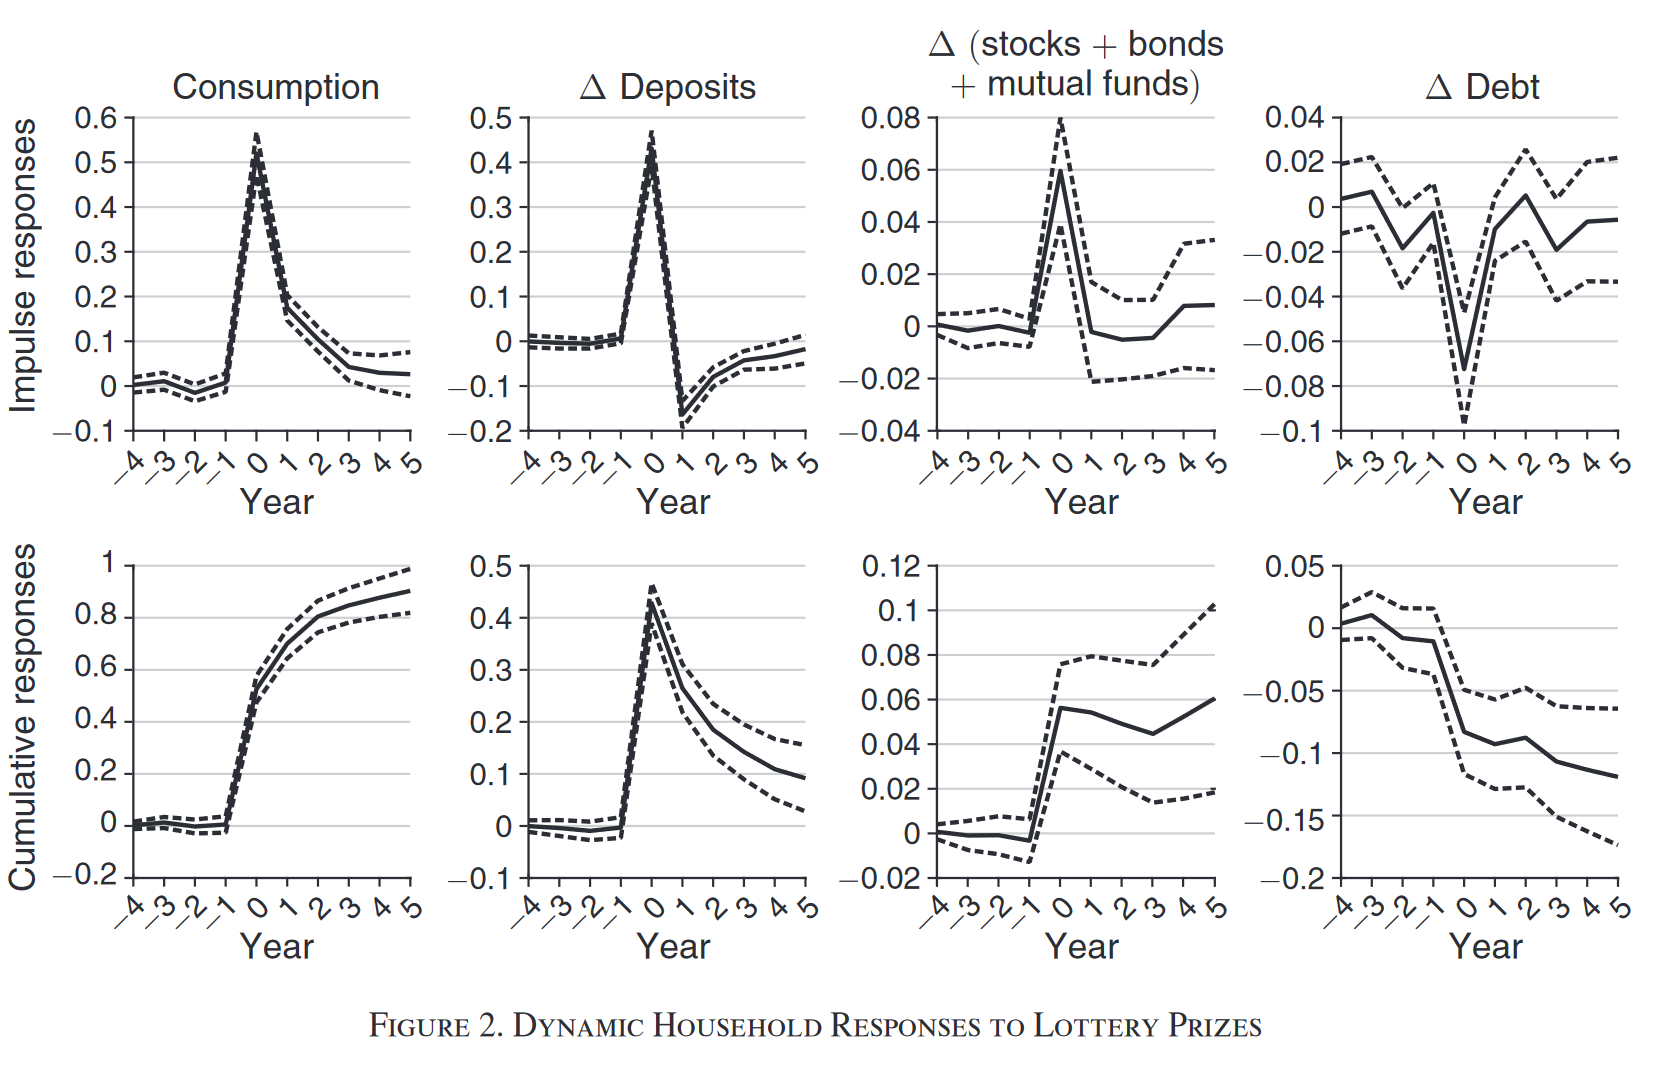
\includegraphics[width=1\textwidth]{figs/Fagereng_MPCs}

\textbf{Source:} Fagereng et al.~(2021). \textbf{PIH says} \(\frac{r}{1+r}\approx2\%\).
\end{frame}

\begin{frame}{What is missing from the model}
\protect\phantomsection\label{what-is-missing-from-the-model}
We make two changes to the PIH model

\begin{enumerate}
\tightlist
\item Introduce uninsurable \textbf{income risk}
\item A \textbf{borrowing constraint}
\end{enumerate}

This gives us:

\begin{enumerate}
\tightlist
\item A precautionary savings motive (on top of consumption smoothing)
\item Higher MPCs when households are close to the borrowing constraint
\item Break the linearity of the consumption function \(\Rightarrow\) distribution starts to matter
\end{enumerate}
\end{frame}

\begin{frame}{Uncertainty and a borrowing constraint}
\protect\phantomsection\label{uncertainty-and-a-borrowing-constraint}
\[
\begin{aligned}
v_{0}(z_{0},a_{-1}) & =\max_{\{c_{t}\}^{\infty}_{t=0}}\mathbb{E}_{0}\left[\sum^{\infty}_{t=0}\beta^{t}u(c_{t})\right]\\
& \text{s.t.}\\
a_{t} & =(1+r)a_{t-1}+wz_{t}-c_{t}  \geq \underline{a} \\
\log z_{t} & = \rho_{z} \log z_{t-1} + \psi_{t},\quad \psi_{t}\sim\mathcal{N}(0,\sigma^{2}_{\psi})\\
\lim_{t\rightarrow\infty}(1+r)^{-t}a_{t} & \geq0\,\,\,\,\,[\text{No-Ponzi game}]
\end{aligned}
\]

\textbf{A true dynamic problem:}

\begin{enumerate}
\tightlist
\item
  \textbf{Information:} \(z_{t}\) is revealed period-by-period
\item
  \textbf{Target:} \emph{Expected} discounted utility,
  \(\mathbb{E}_{0}\left[\sum^{\infty}_{t=0}\beta^{t}u(c_{t})\right]\)
\item
  \textbf{Behavior:} Choose \(c_{t}\) \emph{sequentially} as information
  is revealed
\item
  \textbf{Solution:} Consumption \emph{function},
  \(c^{\ast}(z_{t},a_{t-1})\)
\end{enumerate}
\end{frame}

\begin{frame}{Why is the sequential formulation difficult?}
\protect\phantomsection\label{why-is-the-sequential-formulation-difficult}
\begin{itemize}
\tightlist
\item
  With uncertainty, the optimal sequence is conditional on a given
  realization of shocks
\item
  An optimal sequence should be optimal for every potential realizations
  of shocks!
\item
  Even if \(z_t\) takes only \(\#_{z}\) values, there are \(\#_{z}^{T}\)
  possible histories after \(T\) periods, each with its own consumption
  path \(\Rightarrow\) \textbf{Unfeasible!}
\end{itemize}

This is where \textbf{dynamic programming} becomes necessary
\end{frame}

\begin{frame}{Recursive formulation}
\protect\phantomsection\label{recursive-formulation}
\[
\begin{aligned}
v(z_{t},a_{t-1}) & =\max_{c_{t}}u(c_{t})+\beta\mathbb{E}_{t}\left[v(z_{t+1},a_{t})\right]\\
& \text{s.t. }a_{t}=(1+r)a_{t-1}+wz_{t}-c_{t}\geq\underline{a}
\end{aligned}
\]

\begin{enumerate}
\tightlist
\item
  \textbf{State variables:} \(z_{t}\) \emph{and} \(a_{t-1}\)
\item
  \textbf{Control} (choice) \textbf{variable:} \(c_{t}\)
\item
  \textbf{Continuation value:} \(\beta\mathbb{E}_{t}[v(z_{t+1},a_{t})]\)
\item
  \textbf{Parameters:} \(r\), \(w\), and stuff in \(u(\bullet)\)
\end{enumerate}

\textbf{Note:} no time subscript on \(v\). The problem is stationary, so
the policy function is the same in every period.
\end{frame}

\begin{frame}{IBC}
\protect\phantomsection\label{ibc-1}
\begin{itemize}
\item
  \textbf{Substitution} still implies (path-by-path, for any realization
  of \(z_{t}\)):

  \[
    \begin{aligned}
    R^{-(T-1)}a_{T-1}=0 & \Leftrightarrow & \sum^{T-1}_{t=0}R^{-t}c_{t}=s_{0}+h_{0}
    \end{aligned}
    \]
\item
  \textbf{What if \(T\rightarrow\infty\)?} We must have
  \(\lim_{T\rightarrow\infty}R^{-(T-1)}a_{T-1}=0\)

  \begin{enumerate}
  \tightlist
  \item
    \(\lim_{T\rightarrow\infty}R^{-(T-1)}a_{T-1}>0\): Consumption can be
    increased
  \item
    \(\lim_{T\rightarrow\infty}R^{-(T-1)}a_{T-1}<0\): Violates No-Ponzi
    game condition
  \end{enumerate}
\item
  For \(T\rightarrow\infty\) we have the \textbf{IBC}: \[
    \sum^{\infty}_{t=0}R^{-t}c_{t}=Ra_{-1}+\sum^{\infty}_{t=0}R^{-t}wz_{t}
    \]
\end{itemize}
\end{frame}

\begin{frame}{Natural borrowing limit}
\protect\phantomsection\label{natural-borrowing-limit}
What is the lowest possible value of \(\underline{a}\)?

\begin{itemize}
\item
  Denote \textbf{minimum possible productivity} by
  \textbf{\(\underline{z}\)}
\item
  \textbf{Consumption must be non-negative} \(\Rightarrow\)\\
  \emph{interest payments must be less than minimum income}

  \[
    c_{t}\geq0\Rightarrow r(-a_{t})\leq w\underline{z}\Leftrightarrow a_{t}\geq-\frac{w\underline{z}}{r}
    \]

  If debt was larger it would in the worst case
  (\(\forall z_{t}=\underline{z}\)) grow without bound even with zero
  consumption (\(\forall c_{t}=0\))

  \[
    \begin{aligned}
    a_{0} & =-\frac{w\underline{z}}{r}-\Delta\\
    a_{1} & =(1+r)a_{0}+w\underline{z}=-\frac{w\underline{z}}{r}-(1+r)\Delta\\
    a_{2} & =(1+r)a_{1}+w\underline{z}=-\frac{w\underline{z}}{r}-(1+r)^{2}\Delta\\
    \vdots
    \end{aligned}
    \] \textbf{Natural borrowing constraint:
  \(a_{t}\geq\underline{a}=-\frac{w\underline{z}}{r}\)}
\end{itemize}
\end{frame}

\begin{frame}{Euler-equation with an occasionally binding constraint}
\protect\phantomsection\label{euler-equation-with-an-occasionally-binding-constraint}
\begin{itemize}
\item
  Write the \textbf{Lagrangian} \[
    \mathcal{L}=\frac{c_{t}^{1-\sigma}}{1-\sigma}  +\beta \mathbb{E}_{t}\left[v(z_{t+1},a_{t})\right]+\mu_{t}(a_{t}-\underline{a})
    \] Then: \[
    \begin{aligned}
    \text{FOC:} & \,\,\,c^{-\sigma}_{t}=\beta\mathbb{E}_{t}\left[v_{a}(z_{t+1},a_{t})\right]+\mu_{t}\\
    \text{Slackness:} & \,\,\,\mu_{t}\left(a_{t}-\underline{a}\right)=0\\
    \text{Envelope:} & \,\,\,v_{a}(z_{t},a_{t-1})=(1+r)c^{-\sigma}_{t}
    \end{aligned}
    \]
\item
  \textbf{Two cases:}

  \begin{enumerate}
  \tightlist
  \item
    \textbf{Unconstrained} (\(a_{t}>\underline{a}\), so \(\mu_{t}=0\)):
    \[
     c^{-\sigma}_{t}=\beta R\,\mathbb{E}_{t}\left[c^{-\sigma}_{t+1}\right]
     \]
  \item
    \textbf{Constrained} (\(a_{t}=\underline{a}\), so \(\mu_{t}>0\)): \[
     c^{-\sigma}_{t}>\beta R\,\mathbb{E}_{t}\left[c^{-\sigma}_{t+1}\right]\,\,\,\text{and}\,\,\,c_{t}=(1+r)a_{t-1}+wz_{t}-\underline{a}
     \]
  \end{enumerate}
\end{itemize}
\end{frame}

\begin{frame}{Prudence and precautionary saving}
\protect\phantomsection\label{prudence-and-precautionary-saving}
\begin{itemize}
\item
  \textbf{Prudence:} \(u^{\prime\prime\prime}(c)>0\), i.e.~marginal
  utility is \emph{convex} CRRA has
  \(u^{\prime\prime\prime}(c)=\sigma(\sigma+1)c^{-\sigma-2}>0\)
\item
  \textbf{Jensen on the Euler-equation} (take \(\beta R=1\),
  unconstrained):

  \[
    u^{\prime}(c_{t})=\mathbb{E}_{t}\left[u^{\prime}(c_{t+1})\right]>u^{\prime}\left(\mathbb{E}_{t}\left[c_{t+1}\right]\right)\Leftrightarrow\mathbb{E}_{t}\left[c_{t+1}\right]>c_{t}
    \]
\item
  \textbf{Interpretation:} the household \emph{tilts consumption into
  the future} to build a buffer. Risk lowers consumption today even with
  no constraint.
\item
  \textbf{Two distinct channels, same direction:}

  \begin{enumerate}
  \tightlist
  \item
    \textbf{Risk} \(\times\) \textbf{prudence:} precautionary saving
  \item
    \textbf{Borrowing constraint:} cannot smooth downwards
  \end{enumerate}
\end{itemize}
\end{frame}

\begin{frame}{Special case I: Quadratic utility}
\protect\phantomsection\label{special-case-i-quadratic-utility}
\begin{itemize}
\item
  \textbf{Quadratic utility:}
  \(u(c_{t})=-\frac{1}{2}(\overline{c}-c_{t})^{2}\) with \(\beta R=1\)
  and ``large'' \(\overline{c}\)
\item
  \textbf{Euler-equation:} \emph{Consumption = expected future
  consumption} \[
    \begin{aligned}
    (\overline{c}-c_{t}) & =\mathbb{E}_{t}\left[(\overline{c}-c_{t+k})\right]\Leftrightarrow c_{t}=\mathbb{E}_{t}\left[c_{t+k}\right]
    \end{aligned}
    \]
\item
  Use \textbf{IBC} in expectation to get \textbf{consumption function:}

  \[
    \begin{aligned}
    \sum_{s=0}^{\infty}R^{-s}\mathbb{E}_{0}\left[c_{s}\right] &=Ra_{-1}+\sum_{s=0}^{\infty}R^{-s}w\mathbb{E}_{0}\left[z_{s}\right]\Rightarrow\\
    c^{\ast}(z_{0},a_{-1})=c_{0} &=ra_{-1}+\frac{r}{R}\sum_{s=0}^{\infty}R^{-s}w\mathbb{E}_{0}\left[z_{s}\right]
    \end{aligned}
    \]

  where we formally disregard the borrowing constraint
\item
  \textbf{Certainty equivalence:} \emph{Only expected income matters}.
  No prudence: \(u^{\prime\prime\prime}=0\).
\end{itemize}
\end{frame}

\begin{frame}{Special case II: CARA utility}
\protect\phantomsection\label{special-case-ii-cara-utility}
\begin{itemize}
\item
  \textbf{CARA utility:} \(u(c_{t})=-\frac{1}{\alpha}e^{-\alpha c_{t}}\)
\item
  \textbf{Productivity is absolute random walk:} \[
    z_{t}  =z_{t-1}+\psi_{t}, \quad \psi_{t}  \sim\mathcal{N}(0,\sigma^{2}_{\psi})
    \]
\item
  \textbf{Consumption function}
  (\href{https://www.econ2.jhu.edu/people/ccarroll/public/LectureNotes/Consumption/CARAModelWithYRisk/}{see
  proof})\textbf{:}

  \[
    c^{\ast}(z_{t},a_{t-1})=ra_{t-1}+wz_{t}-\frac{\frac{1}{\alpha}\log\left(\beta R\right)+\frac{\alpha w^{2}\sigma^{2}_{\psi}}{2}}{r}
    \]

  where we formally disregard the borrowing constraint
\item
  \textbf{Precautionary saving:} \(\sigma^{2}_{\psi}\uparrow\) implies
  \(c^{\ast}_{t}\downarrow\) for given \(z_{t}\) and \(a_{t-1}\)

  \(\Rightarrow\) \emph{accumulation of buffer-stock}
\item
  \textbf{But:} the MPC is still \emph{constant}. To solve the problem
  with a more interesting utility function, we need a computer.
\end{itemize}
\end{frame}

\section{VFI applied to the Buffer Stock
Model}\label{vfi-applied-to-the-buffer-stock-model}

\begin{frame}{VFI with uncertainty}
\protect\phantomsection\label{vfi-with-uncertainty}
Uncertainty brings three new difficulties:

\begin{enumerate}
\tightlist
\item
  \textbf{The state space is larger:} loop over all \(a_{t-1}\)
  \textbf{and} all \(z_t\) \pause\\
  With \(\#_{a}\) and \(\#_{z}\) grid points, that is
  \(\#_{a}\times \#_{z}\) maximizations\\
  \(\to\) the cost grows exponentially with the number of states: the
  \textbf{curse of dimensionality} \pause
\item
  \textbf{\(z_t\) is continuous:} we need to discretize the AR(1)
  \pause\\
  A routine gives a grid \(\mathcal{G}_{z}\) and a transition matrix
  \(\Pi_{z}\), \(\pi_{i_{z},i_{z+}}=\Pr[z^{i_{z+}}\,|\,z^{i_{z}}]\)
  \pause
\item
  \textbf{The continuation value is an expectation}
  \(\mathbb{E}_{t}\left[v(z_{t+1},a_{t})\right]\) \pause\\
  Costs \(\#_{z}\) interpolations for \emph{every} trial value of
  \(c_t\) in the maximization
\end{enumerate}
\end{frame}

\begin{frame}[fragile]{Discretizing an AR(1)}
\protect\phantomsection\label{discretizing-an-ar1}
\begin{itemize}
\tightlist
\item
  \textbf{Income process:} \[
    \log z_{t}=\rho_{z}\log z_{t-1}+\psi_{t},\,\,\,\psi_{t}\sim\mathcal{N}(0,\sigma^{2}_{\psi}),\,\,\,\mathbb{E}\left[z_{t}\right]=1
    \]
\item
  \textbf{Tauchen (1986):} evenly spaced grid spanning the unconditional
  distribution, match the transition probabilities by integrating the
  normal density
\item
  \textbf{Rouwenhorst (1995):} build the transition matrix by recursion,
  matching the persistence and the unconditional variance \emph{exactly}

  \begin{itemize}
  \tightlist
  \item
    Preferred at high \(\rho_{z}\), where Tauchen needs many nodes
  \end{itemize}
\item
  In both cases, it gives us:

  \begin{enumerate}
  \tightlist
  \item
    A discretized grid for \(z_t\)
  \item
    A Markov transition matrix \(\Pi_{z}\) with entries
    \(\pi_{i_{z},i_{z+}}\)
  \end{enumerate}
\end{itemize}

Use built-in functions in \textbf{ConSav:}
\texttt{markov.log\_rouwenhorst}, \texttt{markov.tauchen}
\end{frame}

\begin{frame}{Discretizing an AR(1)}
\protect\phantomsection\label{discretizing-an-ar1-1}
\vspace{-4mm}

\begin{center}
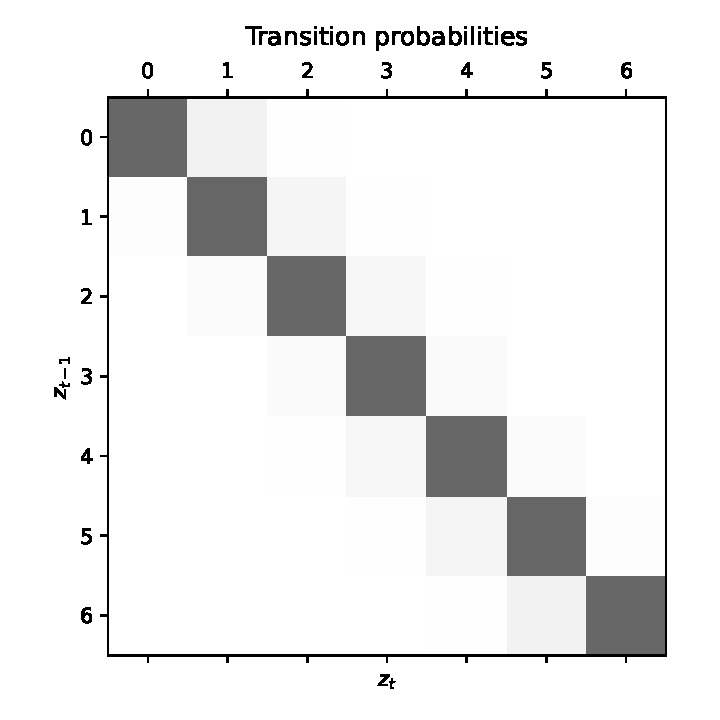
\includegraphics[width=0.6\textwidth]{figs/bs_z_trans}
\end{center}
\end{frame}

\begin{frame}[fragile]{Recursive formulation with \(\underline{v}\)}
\protect\phantomsection\label{recursive-formulation-with-underlinev}
\begin{itemize}
\item
  One useful trick: precompute the \textbf{beginning-of-period value
  function} (of period \(t+1\), before \(z_{t+1}\) is drawn)

  \[
    \underline{v}\left(z_{t},a_{t}\right)=\mathbb{E}_{t}\left[v(z_{t+1},a_{t})\right]=\sum^{\#_{z}-1}_{i_{z+}=0}\pi_{i_{z},i_{z+}}\,v(z^{i_{z+}},a_{t})
    \]
\item
  \textbf{Value function}:

  \[
    \begin{aligned}
    v(z_{t},a_{t-1}) & =\max_{c_{t}}u(c_{t})+\beta\underline{v}\left(z_{t},a_{t}\right)\\
    & \text{s.t. }a_{t}=(1+r)a_{t-1}+wz_{t}-c_{t}\geq\underline{a}
    \end{aligned}
    \]
\item
  \textbf{Why do this?} \emph{Only one interpolation per guess of
  \(c_{t}\)}

  Integrating \emph{inside} the maximization would cost \(\#_{z}\)
  interpolations per guess.
\item
  \textbf{This is the convention} \texttt{GEModelTools} \textbf{uses
  from the next lecture on}
\end{itemize}
\end{frame}

\begin{frame}{}
\protect\phantomsection\label{section-3}
\begin{center}
\LARGE Let's code!
\end{center}
\end{frame}

\begin{frame}{Consumption function}
\protect\phantomsection\label{consumption-function}
\begin{center}
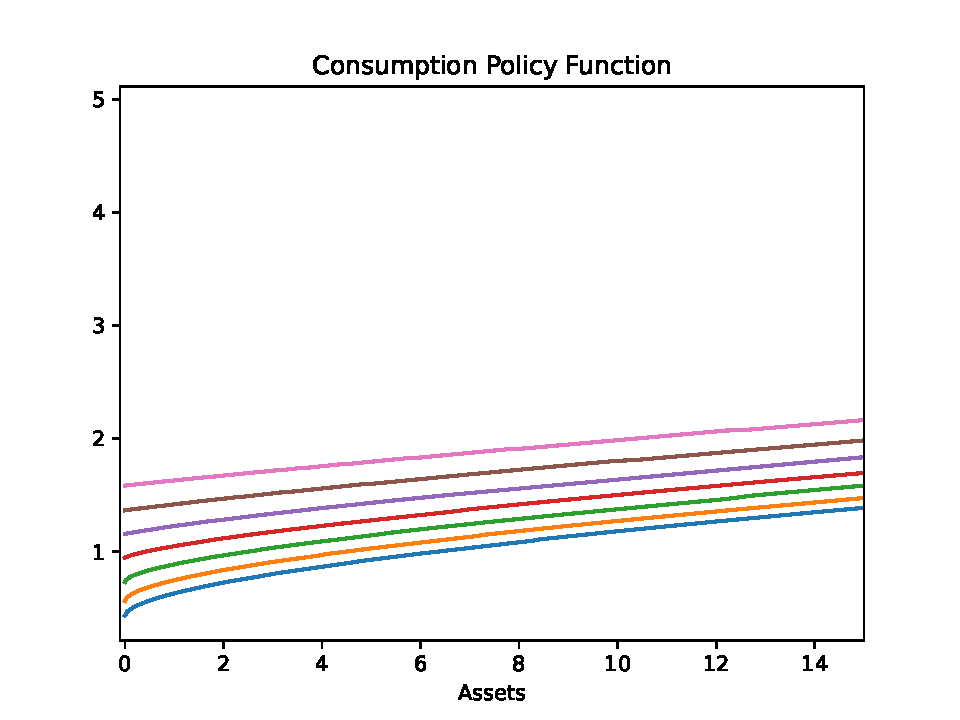
\includegraphics[width=\textwidth]{figs/bs_c_func}
\end{center}
\end{frame}

\begin{frame}{Net savings and the buffer-stock target}
\protect\phantomsection\label{net-savings-and-the-buffer-stock-target}
\begin{center}
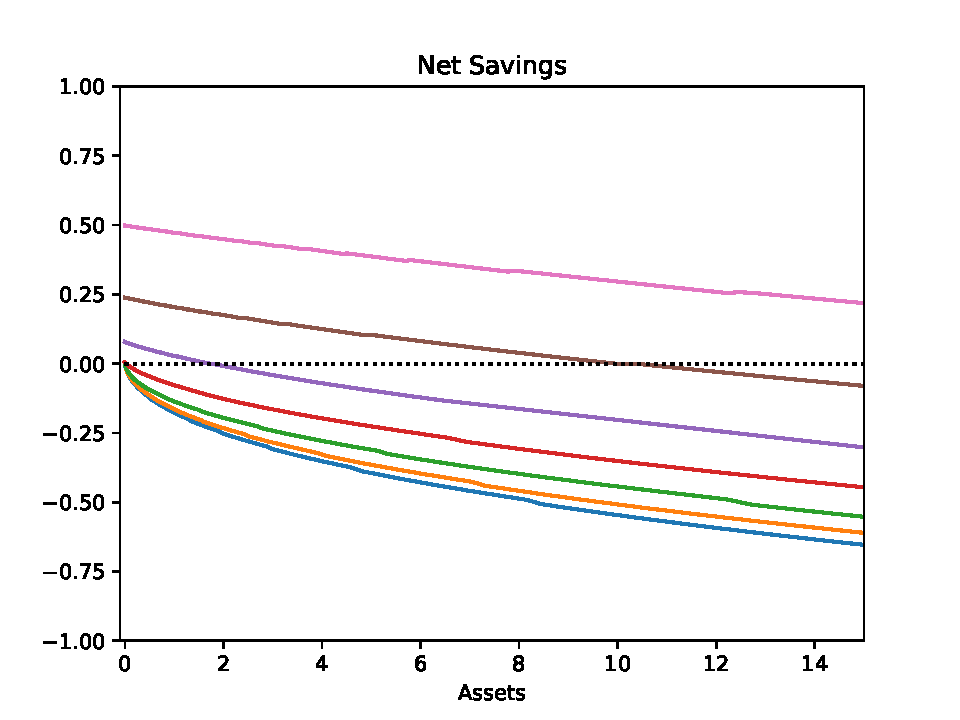
\includegraphics[width=\textwidth]{figs/bs_a_func}
\end{center}

\textbf{Decreasing in wealth and crossing zero:} the crossing point is
the target. It exists despite \(\beta R<1\).
\end{frame}

\begin{frame}{One household, simulated}
\protect\phantomsection\label{one-household-simulated}
\begin{center}
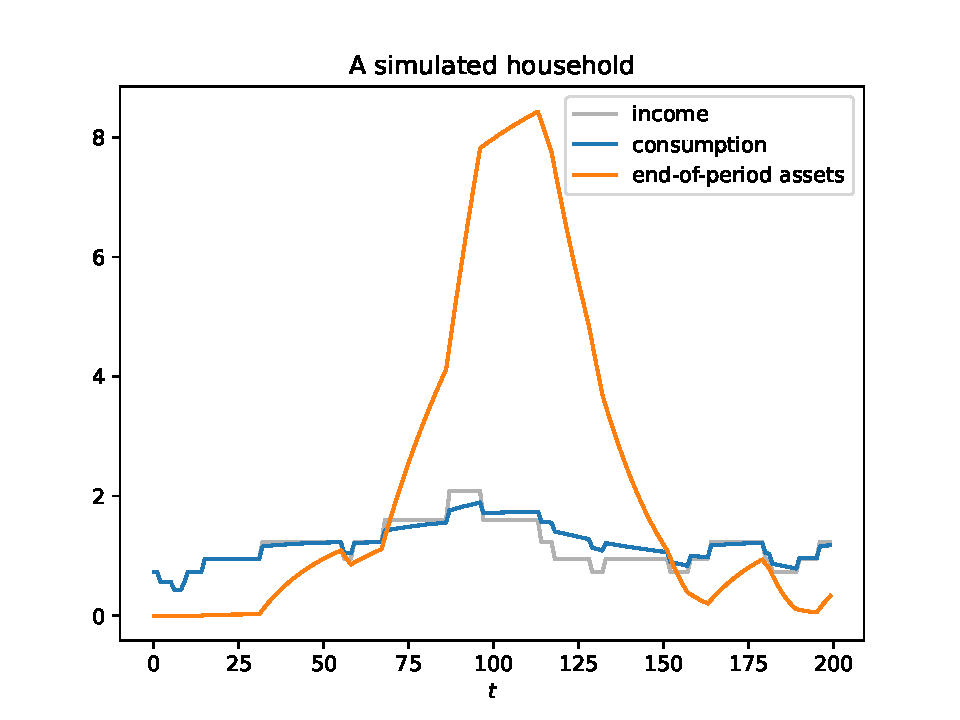
\includegraphics[width=\textwidth]{figs/bs_simulation}
\end{center}
\end{frame}

\begin{frame}{MPC}
\protect\phantomsection\label{mpc}
\begin{center}
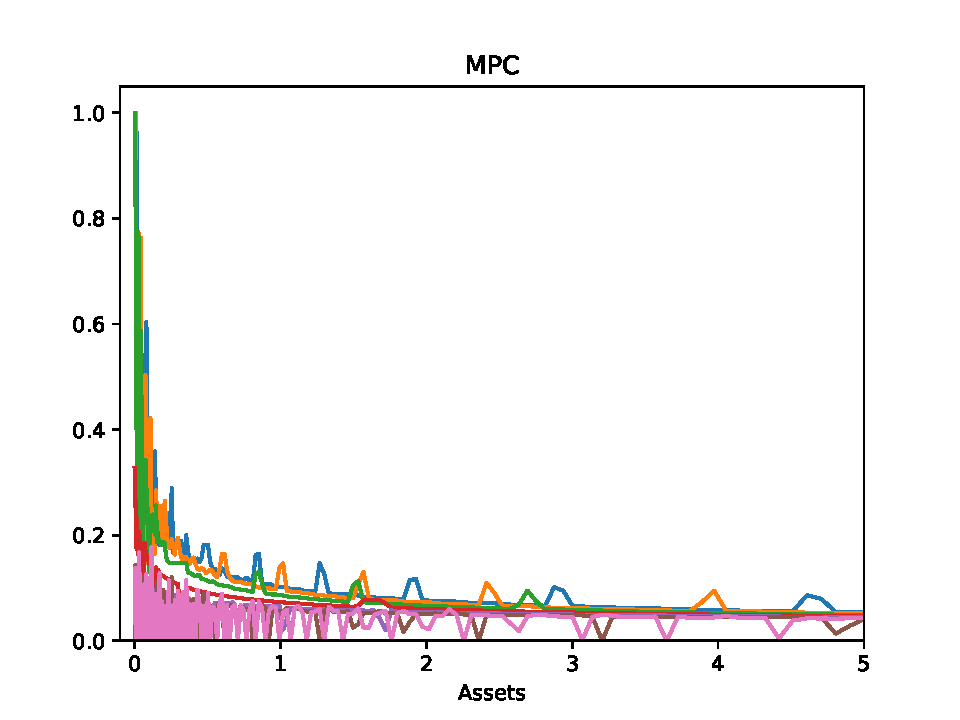
\includegraphics[width=0.72\textwidth]{figs/bs_MPC}
\end{center}

\textbf{One at the constraint, falling steeply with assets.} Under the
PIH it was \(\frac{r}{1+r}\) for everybody.
\end{frame}

\begin{frame}{Economic insights}
\protect\phantomsection\label{economic-insights}
\begin{itemize}
\tightlist
\item
  \textbf{Consumption lower than under PIH and concave in assets}
  \textbf{Intuition:} \emph{Precautionary saving motive is relatively
  larger for asset poor households because income risk is the same for
  everybody} \textbf{Implications:}

  \begin{enumerate}
  \tightlist
  \item
    Windfall gives safety and increases average consumption\\
    \(\Rightarrow\) MPC decreasing in assets
  \item
    Attraction towards a buffer-stock target \(a_{t}=a_{t-1}\) despite
    \(\beta R<1\)
  \item
    Larger effective discounting of future income (extreme: no effect of
    future income changes if constrained before)
  \end{enumerate}
\end{itemize}
\end{frame}

\section{EGM}\label{egm}

\begin{frame}{We can do better}
\protect\phantomsection\label{we-can-do-better}
\begin{itemize}
\tightlist
\item
  We can do better! We know that an optimal consumption choice must
  satisfy the Euler equation, so let's use this
\item
  Great thing about this method: don't need a maximization step, just
  interpolation
\item
  We use information about FOC of the problem: we get a more accurate
  solution
\end{itemize}
\end{frame}

\begin{frame}{Overview of EGM}
\protect\phantomsection\label{overview-of-egm}
\begin{itemize}
\tightlist
\item
  Assume you have a guess on the consumption function,
  \(c^{n}(z_{t},a_{t-1})\). The envelope condition gives
  \(v_{a}=(1+r)c^{-\sigma}\), so on a grid of \emph{end-of-period}
  assets \(a_{t}\) we can compute the marginal beginning-of-period value
  \[
  \underline{v}_{a}(z_{t},a_{t})\equiv \mathbb{E}_{t}\left[v_{a}(z_{t+1},a_{t})\right] = (1+r)\sum^{\#_{z}-1}_{i_{z+}=0}\pi_{i_{z},i_{z+}}\,c^{n}(z^{i_{z+}},a_{t})^{-\sigma}
  \]
\item
  Then back out the state that makes \(a_{t}\) optimal, from the FOC and
  the budget constraint: \[\begin{aligned}
    c_{t}^{-\sigma} &= \beta\,\underline{v}_{a}(z_{t},a_{t}) \\
    \big((1+r)a_{t-1}+wz_{t}-a_{t}\big)^{-\sigma} &= \beta\,\underline{v}_{a}(z_{t},a_{t}) \\
    a_{t-1}(z_{t},a_{t}) &= \frac{\big(\beta\,\underline{v}_{a}(z_{t},a_{t})\big)^{-\frac{1}{\sigma}}+a_{t}-w z_{t}}{1+r}
  \end{aligned}\]
\end{itemize}
\end{frame}

\begin{frame}{Overview of EGM (continued)}
\protect\phantomsection\label{overview-of-egm-continued}
\begin{itemize}
\tightlist
\item
  This is why it's called the \textbf{endogenous grid method}: we get an
  endogenous grid of states \(a_{t-1}\) for a fixed grid of choices
  \(a_t\)
\item
  Interpolate to invert the mapping and get \(a^{\ast}(z_t,a_{t-1})\) on
  the exogenous grid. If \(a^{\ast}(z_t,a_{t-1})< \underline{a}\), set
  \(a^{\ast}=\underline{a}\) to enforce the borrowing constraint
\item
  Iterate until convergence, done!
\end{itemize}
\end{frame}

\begin{frame}{}
\protect\phantomsection\label{section-4}
\begin{center}
\LARGE Let's code!
\end{center}
\end{frame}

\begin{frame}{VFI vs EGM}
\protect\phantomsection\label{vfi-vs-egm}
\begin{tabular}{@{}c@{\hspace{2mm}}c@{}}
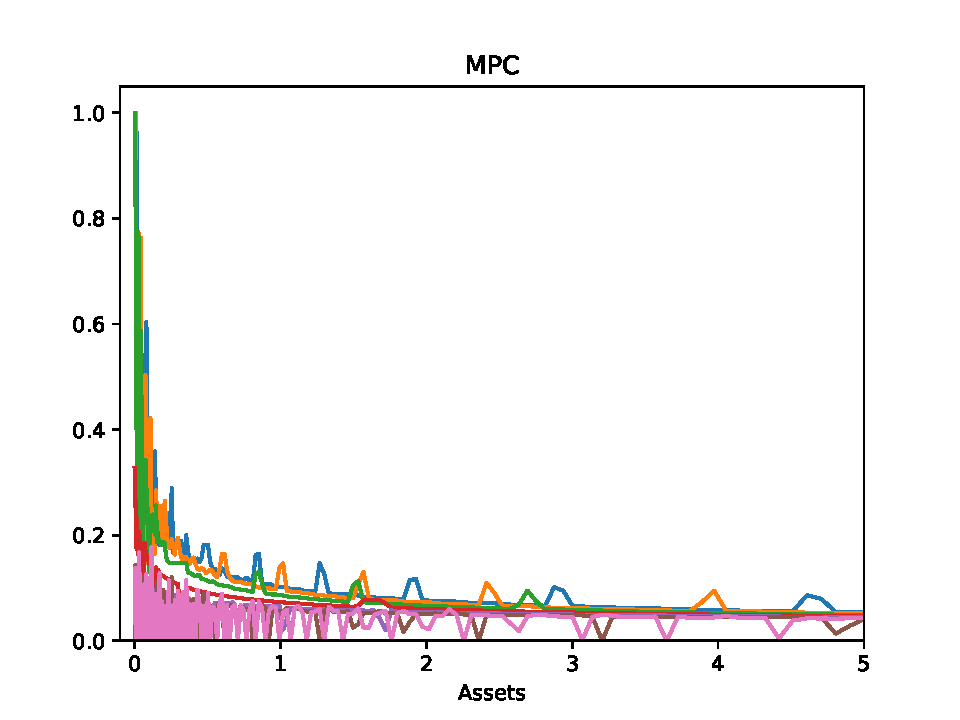
\includegraphics[width=0.48\textwidth]{figs/bs_MPC} & 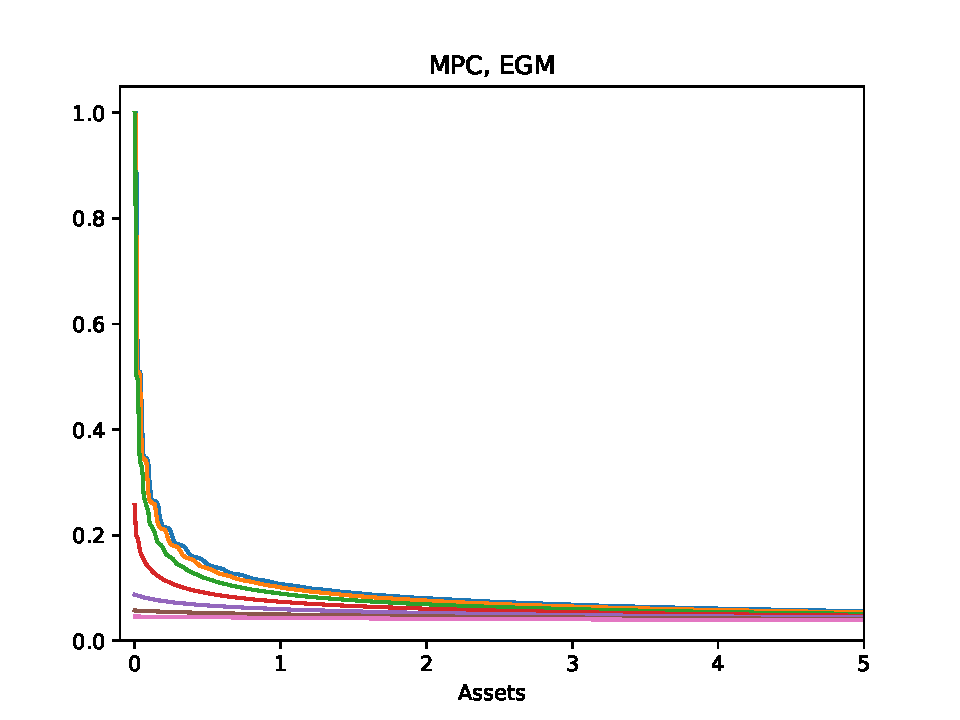
\includegraphics[width=0.48\textwidth]{figs/egm_MPC}\tabularnewline
\end{tabular}
\end{frame}

\begin{frame}[fragile]{Exercise: permanent productivity types}
\protect\phantomsection\label{exercise-permanent-productivity-types}
\begin{itemize}
\tightlist
\item
  \textbf{Add permanent types:} \(\xi\in\{0.5,1,1.5\}\), fixed for life, income \(w\xi z_{t}\)
\item
  \textbf{Write} \texttt{solve\_hh\_backwards\_fix} with the extra leading dimension, \texttt{a[i\_fix,i\_z,:]}, exactly the layout of \texttt{household\_problem.py} in lecture 04
\item
  \textbf{Plot} the consumption functions of the three types
\item
  \textbf{Check homogeneity:} with CRRA and \(\underline{a}=0\),
  \[
  c^{\ast}(z,a_{-1};\xi)=\xi\,c^{\ast}(z,a_{-1}/\xi;1)
  \]
  What does it imply for wealth-to-income ratios across types?
\end{itemize}

\vspace{2mm}

\textbf{Notebook:} \texttt{04\_egm.ipynb}, last section
\end{frame}

\section{Simulation and aggregation}\label{simulation-and-aggregation}

\begin{frame}[fragile]{From policy functions to aggregates}
\protect\phantomsection\label{from-policy-functions-to-aggregates}
\begin{itemize}
\item
  \textbf{What we have:} \(c^{\ast}(z_{t},a_{t-1})\) and
  \(a^{\ast}(z_{t},a_{t-1})\), what \emph{one} household does in every
  state
\item
  \textbf{What the next lecture needs:} aggregates, e.g.\vspace{-1mm}

  \[
    A^{hh}_{t}=\sum_{i_{z}}\sum_{i_{a-}}\boldsymbol{D}_{t}(z^{i_{z}},a^{i_{a-}})\,a^{\ast}(z^{i_{z}},a^{i_{a-}})
    \]

  where \(\boldsymbol{D}_{t}\) is the \emph{distribution} of households
  over \(\mathcal{G}_{z}\times\mathcal{G}_{a}\)
\item
  \textbf{So we need to simulate the distribution forward.} Two ways:

  \begin{enumerate}
  \tightlist
  \item
    Monte Carlo: simulate \(N\) households, average
  \item
    Histogram (Young, 2010): iterate on \(\boldsymbol{D}_{t}\) itself
  \end{enumerate}
\item
  \textbf{Notebook:} \texttt{05\textbackslash{}\_simulation.ipynb}
\end{itemize}
\end{frame}

\begin{frame}{Monte Carlo simulation}
\protect\phantomsection\label{monte-carlo-simulation}
\begin{itemize}
\tightlist
\item
  \textbf{Initial distribution:} draw \(z_{i,-1}\) and \(a_{i,-1}\) for
  \(i\in\{0,1,\dots,N-1\}\)
\item
  \textbf{Simulation:} forwards in time from \(t=0\), in each period

  \begin{enumerate}
  \item
    Draw \(z_{it}\) given \(z_{it-1}\) from the transition probabilities
  \item
    Use linear interpolation to evaluate\vspace{-1mm}

    \[
     a_{it}=a^{\ast}(z_{it},a_{it-1})
     \]
  \end{enumerate}
\item
  \textbf{Aggregation:} sample averages,
  \(A^{hh}_{t}=\frac{1}{N}\sum_{i}a_{it}\)

  \begin{itemize}
  \tightlist
  \item
    Law of large numbers: correct as \(N\rightarrow\infty\)
  \end{itemize}
\item
  \textbf{Pro:} simple to implement, works for any model
\item
  \textbf{Con:} computationally costly, and \emph{random}
\end{itemize}
\end{frame}

\begin{frame}{Monte Carlo noise}
\protect\phantomsection\label{monte-carlo-noise}
\begin{tabular}{@{}c@{\hspace{2mm}}c@{}}
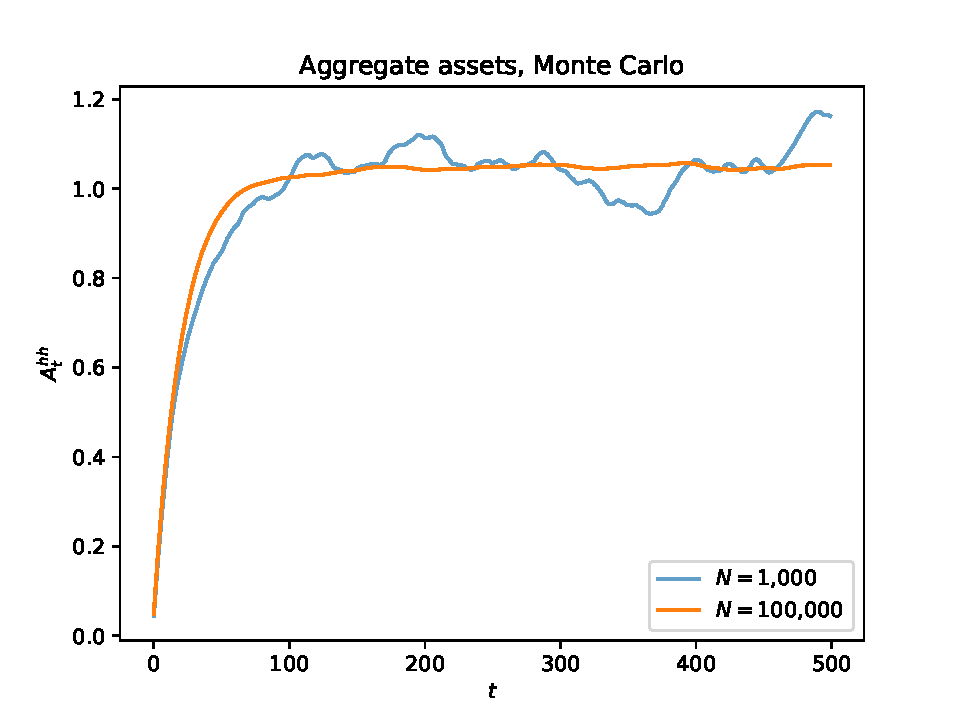
\includegraphics[width=0.48\textwidth]{figs/sim_mc_A} & 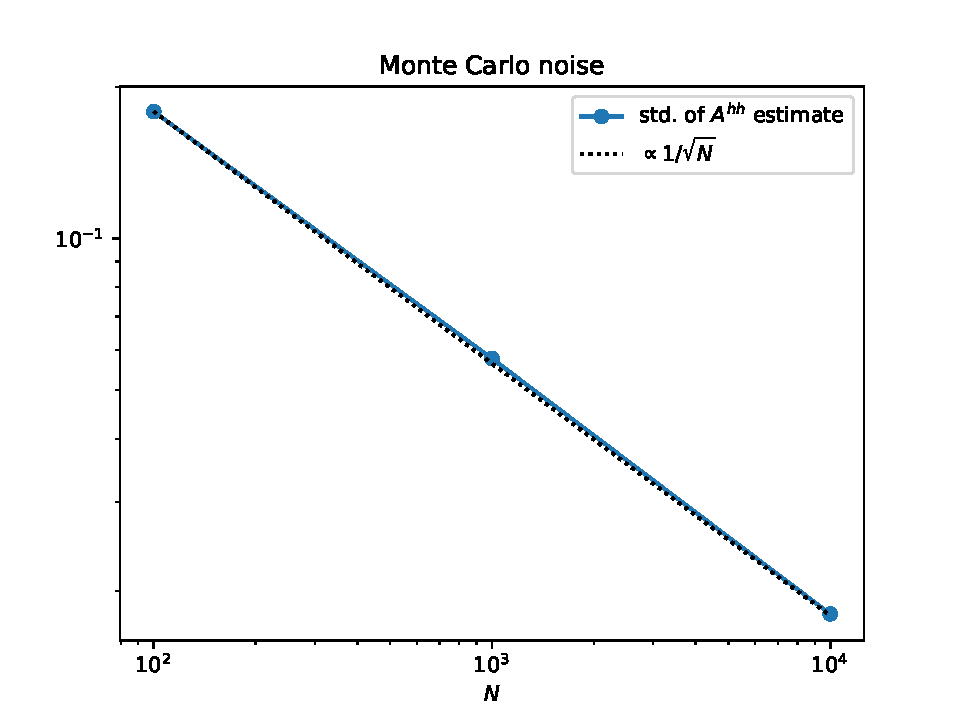
\includegraphics[width=0.48\textwidth]{figs/sim_mc_noise}\tabularnewline
\end{tabular}

\vspace{-1mm}

\begin{itemize}
\tightlist
\item
  \textbf{Left:} \(A^{hh}_{t}\) never settles, it keeps fluctuating
  around its stationary level
\item
  \textbf{Right:} the error falls like \(1/\sqrt{N}\): quadrupling \(N\)
  halves it
\item
  \textbf{Why this hurts:} next lecture we root-find on asset market
  clearing, \(A^{hh}(r)-K(r)=0\). A stochastic \(A^{hh}\) puts a floor
  on the achievable tolerance
\end{itemize}
\end{frame}

\begin{frame}{The distribution as an object}
\protect\phantomsection\label{the-distribution-as-an-object}
\begin{itemize}
\item
  \textbf{Idea:} stop tracking households, track \emph{probability mass}
\item
  \textbf{Histogram:} an array \(\boldsymbol{D}\) on
  \(\mathcal{G}_{z}\times\mathcal{G}_{a}\), summing to \(1\)

  \begin{itemize}
  \tightlist
  \item
    \(\underline{\boldsymbol{D}}_{t}\): beginning-of-period, over
    \((z_{t-1},a_{t-1})\)
  \item
    \(\boldsymbol{D}_{t}\): after the productivity draw, over
    \((z_{t},a_{t-1})\)
  \end{itemize}
\item
  \textbf{The productivity transition is exact:}\vspace{-1mm}

  \[
    \boldsymbol{D}_{t}(z^{i_{z}},a^{i_{a-}})=\sum_{i_{z-}}\pi_{i_{z-},i_{z}}\underline{\boldsymbol{D}}_{t}(z^{i_{z-}},a^{i_{a-}})\iff\boldsymbol{D}_{t}=\Pi^{\prime}_{z}\underline{\boldsymbol{D}}_{t}
    \]
\item
  \textbf{The problem:} all mass at \((z^{i_{z}},a^{i_{a-}})\) saves
  \(a^{\ast}(z^{i_{z}},a^{i_{a-}})\), which falls \emph{between} grid
  points
\end{itemize}
\end{frame}

\begin{frame}{The savings lottery}
\protect\phantomsection\label{the-savings-lottery}
\begin{itemize}
\item
  \textbf{Split the mass between the two neighbors.} Find \(i\) such
  that \(a^{i}\leq a^{\ast}\leq a^{i+1}\) and set\vspace{-1mm}

  \[
    \omega=\frac{a^{i+1}-a^{\ast}}{a^{i+1}-a^{i}}\in[0,1]
    \]
\item
  \textbf{Assign} share \(\omega\) to \(a^{i}\) and \(1-\omega\) to
  \(a^{i+1}\)

  \begin{itemize}
  \tightlist
  \item
    The lottery has mean \emph{exactly} \(a^{\ast}\): aggregate savings
    are not distorted by the grid
  \end{itemize}
\item
  \textbf{One full period:}\vspace{-1mm}

  \[
    \underline{\boldsymbol{D}}_{t}\overset{\Pi^{\prime}_{z}}{\longrightarrow}\boldsymbol{D}_{t}\overset{\Lambda^{\prime}}{\longrightarrow}\underline{\boldsymbol{D}}_{t+1}
    \]

  where \(\Lambda\) collects the lottery weights
\item
  \textbf{Both maps are linear and deterministic:} simulation becomes
  matrix algebra. No draws, no noise
\end{itemize}
\end{frame}

\begin{frame}{One period forward, in pictures}
\protect\phantomsection\label{one-period-forward-in-pictures}
\begin{center}
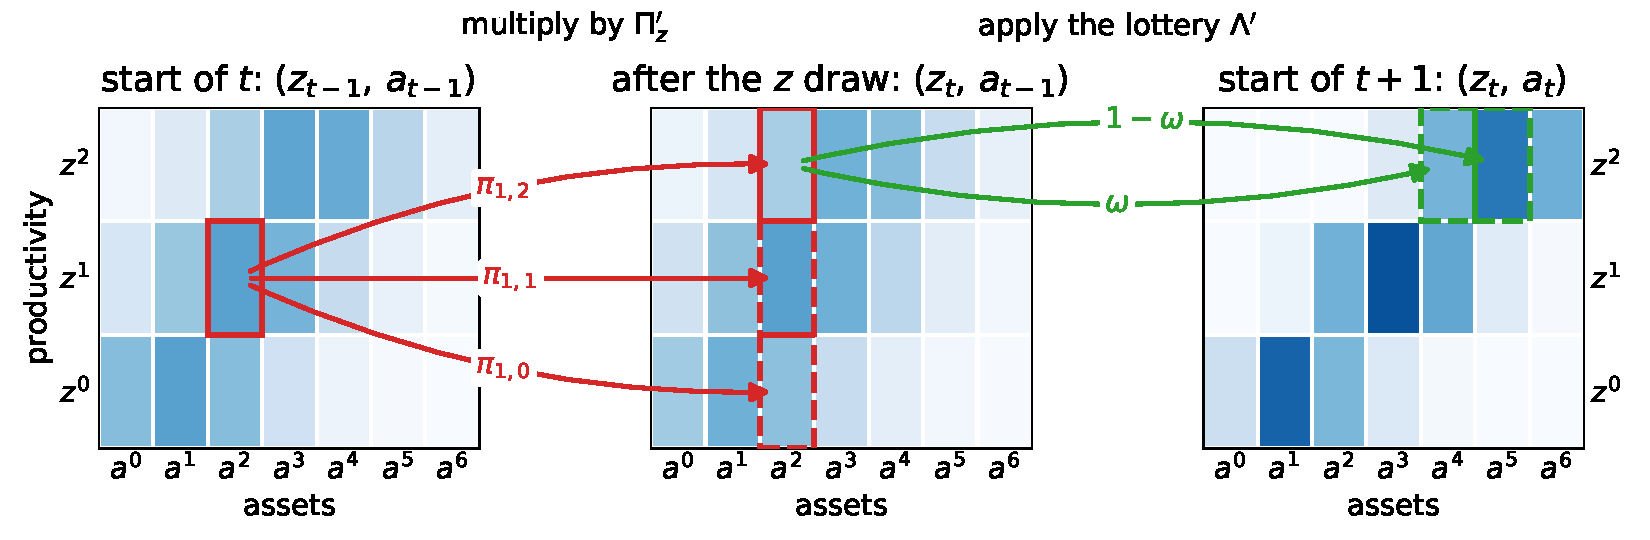
\includegraphics[width=\textwidth]{figs/sim_young_method}
\end{center}

\vspace{-2mm}

\begin{itemize}
\tightlist
\item
  \textbf{Productivity draw:} the mass at \((z^{1},a^{2})\) is spread
  over the column \(a^{2}\), with the weights of row \(1\) of
  \(\Pi_{z}\). Assets do not move
\item
  \textbf{Savings lottery:} those who drew \(z^{2}\) save
  \(a^{\ast}\in[a^{4},a^{5}]\). Their mass moves along the row, split
  \(\omega\) and \(1-\omega\). Productivity does not move
\item
  \textbf{Every cell does both,} and the two maps are the matrices
  \(\Pi_{z}^{\prime}\) and \(\Lambda^{\prime}\)
\end{itemize}
\end{frame}

\begin{frame}{Monte Carlo vs histogram}
\protect\phantomsection\label{monte-carlo-vs-histogram}
\begin{center}
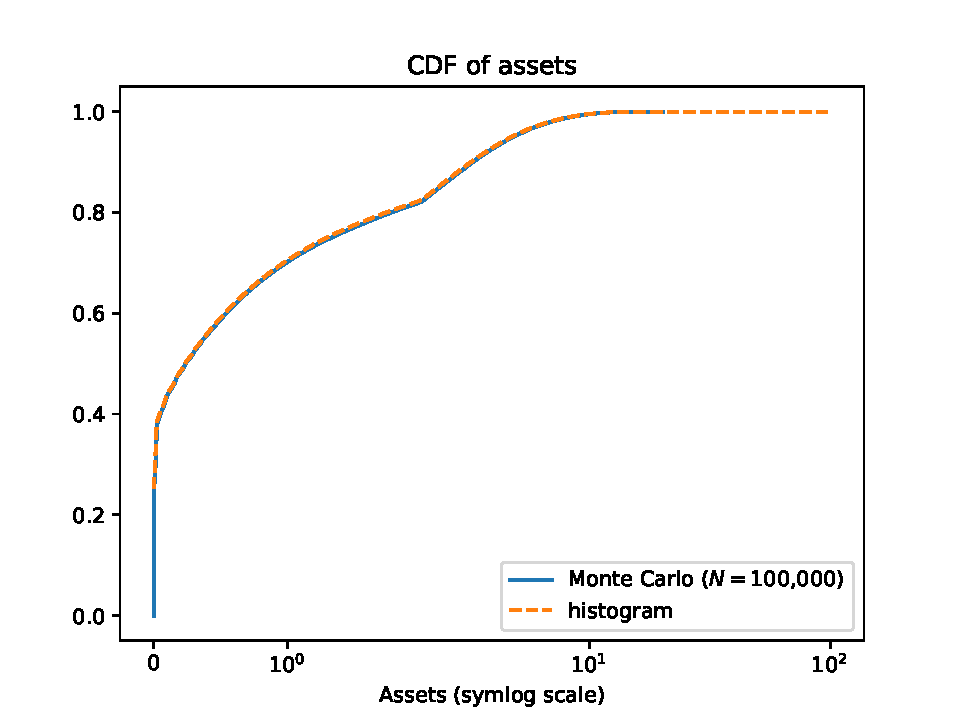
\includegraphics[width=0.72\textwidth]{figs/sim_mc_vs_hist}
\end{center}

\vspace{-2mm}

\textbf{Same distribution.} The histogram is the exact limit the Monte
Carlo approaches by brute force, at a fraction of the cost. Its only
cost: the distribution lives \emph{on the grid}.
\end{frame}

\begin{frame}{Aggregation}
\protect\phantomsection\label{aggregation}
\begin{itemize}
\item
  \textbf{Aggregates are sums over the grid:}\vspace{-1mm}

  \[
    A^{hh}=\sum_{i_{z},i_{a-}}\boldsymbol{D}(z^{i_{z}},a^{i_{a-}})\,a^{\ast}(z^{i_{z}},a^{i_{a-}}),\qquad C^{hh}=\sum_{i_{z},i_{a-}}\boldsymbol{D}\,c^{\ast}
    \]
\item
  \textbf{Stationary distribution:} iterate the forward step until
  \(\underline{\boldsymbol{D}}\) stops moving (526 iterations, \(0.01\)
  secs)
\end{itemize}
\end{frame}

\begin{frame}[fragile]{Exercise: death}
\protect\phantomsection\label{exercise-death}
\begin{itemize}
\tightlist
\item
  \textbf{Perpetual youth:} after saving, die with probability \(\delta=0.02\). Replaced by a newborn with \(a=0\) and ergodic \(z\). No annuities, the assets of the dead are lost.
\item
  \textbf{Backward:} \(\beta\rightarrow\beta(1-\delta)\). No new code, use \texttt{par.\_replace}
\item
  \textbf{Forward:} add a death step to \texttt{simulate\_hh\_forwards}. Where exactly?
\item
  \textbf{Compare} the CDF of assets and \(A^{hh}\) with the baseline
\item
  \(C^{hh}=rA^{hh}+w\) \textbf{now fails.} Derive the identity that replaces it and check it
\end{itemize}

\vspace{2mm}

\textbf{Notebook:} \texttt{05\_simulation.ipynb}, last section
\end{frame}

\section{Recap}\label{recap}

\begin{frame}{Recap I: buffer-stock theory}
\protect\phantomsection\label{recap-i-buffer-stock-theory}
\begin{itemize}
\tightlist
\item
  \textbf{PIH:} consume the annuity value of total wealth, \(\text{MPC}=\frac{r}{1+r}\approx2\%\), consumption linear in wealth, the distribution is irrelevant. \textbf{Data:} \(40\)-\(50\%\).
\item
  \textbf{Two ingredients fix it:} uninsurable income risk and a borrowing constraint.
\item
  \textbf{Euler-equation with an occasionally binding constraint:}
  \[
  u^{\prime}(c_{t})\geq\beta R\,\mathbb{E}_{t}\left[u^{\prime}(c_{t+1})\right],\quad\text{with equality if }a_{t}>\underline{a}
  \]
\item
  \textbf{Prudence} (\(u^{\prime\prime\prime}>0\)) \(\times\) \textbf{risk} \(\Rightarrow\) \textbf{precautionary saving}: consume less today, tilt consumption into the future.
\item
  \textbf{Policy functions:} consumption \emph{concave} in assets. MPC one at the constraint, falling with wealth. Net savings cross zero: a \textbf{buffer-stock target}, even with \(\beta R<1\).
\item
  \textbf{Consequence:} who holds what matters. The aggregate MPC is a property of the \emph{distribution}.
\end{itemize}
\end{frame}

\begin{frame}[fragile]{Recap II: EGM}
\protect\phantomsection\label{recap-ii-egm}
\begin{itemize}
\tightlist
\item
  \textbf{VFI:} an optimizer at every grid point, interpolating the \emph{value} function. Slow and ragged policies.
\item
  \textbf{EGM:} iterate on the Euler-equation, with the grid on the \emph{choice} \(a_{t}\) instead of the state \(a_{t-1}\). Given \(\underline{v}_{a}(z_{t},a_{t})\):

  \begin{enumerate}
  \tightlist
  \item
    Invert the FOC: \(c(z_{t},a_{t})=\left[\beta\underline{v}_{a}(z_{t},a_{t})\right]^{-1/\sigma}\)
  \item
    Endogenous grid from the budget: \(a_{t-1}=\frac{a_{t}+c-wz_{t}}{1+r}\)
  \item
    Interpolate \(a^{\ast}\) back on the fixed grid, impose \(a^{\ast}\geq\underline{a}\), get \(c^{\ast}\) from the budget
  \item
    Envelope + expectation: \(\underline{v}_{a}=\Pi_{z}\left[(1+r)(c^{\ast})^{-\sigma}\right]\)
  \end{enumerate}
\item
  \textbf{No optimizer, one interpolation per} \(z\): \(\approx15\times\) faster per step, same number of steps (contraction with modulus \(\beta\)).
\item
  \textbf{Smoother:} interpolates the \emph{policy} function, which is close to linear. Clean MPCs.
\item
  \texttt{solve\_hh\_backwards} is the backward step of \texttt{GEModelTools}.
\end{itemize}
\end{frame}

\begin{frame}[fragile]{Recap III: the histogram method}
\protect\phantomsection\label{recap-iii-the-histogram-method}
\begin{itemize}
\tightlist
\item
  \textbf{To aggregate we need the distribution} \(\boldsymbol{D}\) over \(\mathcal{G}_{z}\times\mathcal{G}_{a}\).
\item
  \textbf{Monte Carlo:} simulate \(N\) households. Burn-in, and noise \(\propto1/\sqrt{N}\) that never goes away: fatal for root-finding on market clearing.
\item
  \textbf{Histogram (Young, 2010):} track probability mass, not households. Two deterministic transitions:

  \begin{enumerate}
  \tightlist
  \item
    Productivity: \(\boldsymbol{D}_{t}=\Pi_{z}^{\prime}\,\underline{\boldsymbol{D}}_{t}\)
  \item
    Savings lottery: \(a^{\ast}\in[a^{i},a^{i+1}]\), share \(\omega=\frac{a^{i+1}-a^{\ast}}{a^{i+1}-a^{i}}\) to \(a^{i}\), \(1-\omega\) to \(a^{i+1}\). Mean-preserving, so aggregate savings are not distorted.
  \end{enumerate}
\item
  \textbf{Iterate until} \(\boldsymbol{D}\) \textbf{stops moving:} the stationary distribution. Exact given the grid, no random numbers, a fraction of the time.
\item
  \texttt{simulate\_hh\_forwards} is the forward step of \texttt{GEModelTools}.
\end{itemize}
\end{frame}

\begin{frame}{Recap IV: aggregation}
\protect\phantomsection\label{recap-iv-aggregation}
\begin{itemize}
\tightlist
\item
  \textbf{Aggregates are sums over the grid:}
  \[
  A^{hh}=\sum_{i_{z}}\sum_{i_{a-}}\boldsymbol{D}(z^{i_{z}},a^{i_{a-}})\,a^{\ast}(z^{i_{z}},a^{i_{a-}}),\qquad C^{hh}=\sum\boldsymbol{D}\,c^{\ast}
  \]
  with \(\boldsymbol{D}\) \emph{after} the productivity draw, so it lines up with the policy functions.
\item
  \textbf{Check:} in the stationary distribution \(C^{hh}=rA^{hh}+w\).
\item
  \textbf{Aggregate MPC:} \(\sum\boldsymbol{D}\,\text{MPC}\approx0.33\), against \(0.02\) under the PIH. A quarter of households sit at the constraint.
\item
  \textbf{Same recipe next lecture,} but \(r\) and \(w\) will be chosen so that \(A^{hh}\) clears the asset market.
\end{itemize}
\end{frame}

\begin{frame}[fragile]{The household block in practice}
\protect\phantomsection\label{the-household-block-in-practice}
\begin{enumerate}
\item
  \textbf{Backward step (EGM):} iterate\vspace{-1mm}

  \[
   \underline{v}_{a}\rightarrow c^{\ast}(z_{t},a_{t-1}),\,a^{\ast}(z_{t},a_{t-1})
   \]

  until the policy functions converge \(\Rightarrow\)
  \texttt{solve\_hh\_backwards}
\item
  \textbf{Forward step (histogram):} build the lottery from
  \(a^{\ast}\), iterate\vspace{-1mm}

  \[
   \underline{\boldsymbol{D}}_{t}\overset{\Pi^{\prime}_{z}}{\longrightarrow}\boldsymbol{D}_{t}\overset{\Lambda^{\prime}}{\longrightarrow}\underline{\boldsymbol{D}}_{t+1}
   \]

  until the distribution converges \(\Rightarrow\)
  \texttt{simulate\_hh\_forwards}
\item
  \textbf{Aggregate:} \(A^{hh}=\sum\boldsymbol{D}\,a^{\ast}\),
  \(C^{hh}=\sum\boldsymbol{D}\,c^{\ast}\)
\end{enumerate}

\vspace{2mm}

\textbf{This pair is the household block.} Next lecture
\texttt{GEModelTools} runs it for us, and \(r\) and \(w\) become
equilibrium objects.
\end{frame}

\begin{frame}{What you should remember}
\protect\phantomsection\label{what-you-should-remember}
\begin{enumerate}
\tightlist
\item
  \textbf{The PIH gives an MPC of about} \(2\%\)\textbf{; the data say}
  \(40-50\%\)
\item
  \textbf{Uncertainty plus a borrowing constraint fixes it}
\item
  \textbf{EGM solves the household problem fast and accurately}
\item
  \textbf{The histogram method gives a precise distribution,} without
  simulation noise
\end{enumerate}

\textbf{Next:} \emph{Stationary equilibrium}

\textbf{You should:}

\begin{enumerate}
\tightlist
\item
  Study the code from this lecture
\item
  Glance at Aiyagari (1994),``Uninsured Idiosyncratic Risk and Aggregate
  Saving''
\end{enumerate}
\end{frame}

\begin{frame}[fragile]{Exercise: endogenous labor supply}
\protect\phantomsection\label{exercise-endogenous-labor-supply}
\[
v(z_{t},a_{t-1})=\max_{c_{t},n_{t}}\frac{c_{t}^{1-\sigma}}{1-\sigma}-\varphi\frac{n_{t}^{1+\nu}}{1+\nu}+\beta\mathbb{E}_{t}\left[v(z_{t+1},a_{t})\right]
\]
\[
\text{s.t.}\quad a_{t}=(1+r)a_{t-1}+wz_{t}n_{t}-c_{t}\geq0
\]

\begin{enumerate}
\tightlist
\item
  \textbf{FOCs:} show that \(\varphi n_{t}^{\nu}=wz_{t}c_{t}^{-\sigma}\), constrained or not
\item
  \textbf{EGM, unconstrained:} Euler gives \(c\), the intratemporal FOC gives \(n\), the budget gives \(a_{t-1}\). One extra line
\item
  \textbf{EGM, constrained:} \(a^{\ast}=0\), but \(c\) and \(n\) must be found together. Newton on one equation in \(n\)
\item
  \textbf{Policy functions:} does labor supply fall with wealth? With \(z\)?
\item
  \textbf{Simulate and aggregate:} \(L^{hh}=\sum\boldsymbol{D}\,z\,n^{\ast}\), check \(C^{hh}=rA^{hh}+wL^{hh}\). Share at the constraint?
\end{enumerate}

\textbf{Notebook:} \texttt{06\_egm\_endogenous\_labor.ipynb}
\end{frame}

\section{Misc}\label{misc}

\begin{frame}{1. Life-cycle (I)}
\protect\phantomsection\label{life-cycle-i}
\begin{itemize}
\tightlist
\item
  \textbf{Basically:}

  \begin{enumerate}
  \tightlist
  \item
    Born, working, retired, die
  \item
    Age-varying parameters (esp.~income)
  \end{enumerate}
\item
  \textbf{Add-ons:}

  \begin{enumerate}
  \tightlist
  \item
    Labor supply, human capital, occupation
  \item
    Portfolio choice and entrepreneurship
  \item
    Family formation
  \item
    Health, mortality
  \item
    etc.
  \end{enumerate}
\item
  \textbf{Good starting example:} ``Life‐Cycle Consumption and Children:
  Evidence from a Structural Estimation'', Jørgensen (2017)
\end{itemize}
\end{frame}

\begin{frame}{1. Life-cycle (II)}
\protect\phantomsection\label{life-cycle-ii}
\vspace{-2mm}

\begin{columns}[T]
\begin{column}{0.5\linewidth}
\textbf{Paper:} Gourinchas and Parker (2002)

\emph{Life-cycle consumption-saving model with retirement}

\begin{itemize}[<+->]
\item
  Young households:\\
  Save for precautionary reasons (buffer)
\item
  Older households:\\
  Save for retirement (life-cycle)
\end{itemize}
\end{column}

\begin{column}{0.5\linewidth}
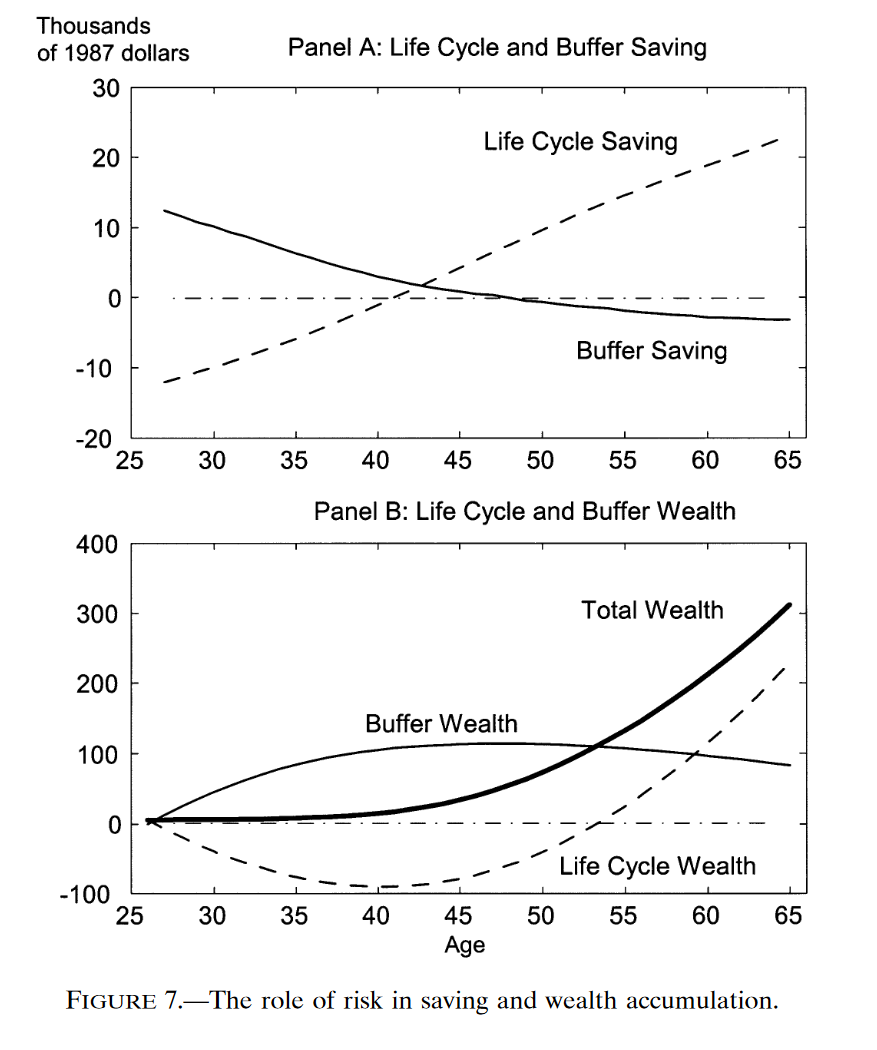
\includegraphics[width=1\textwidth]{figs/GourchasParker}
\end{column}
\end{columns}
\end{frame}

\begin{frame}{1. Life-cycle (III)}
\protect\phantomsection\label{life-cycle-iii}
\begin{itemize}
\tightlist
\item
  \textbf{Natural experiment:} Wealth depletion after sudden inheritance
\item
  \textbf{Results:}

  \begin{enumerate}
  \tightlist
  \item
    Life-cycle profile of wealth fitted for many levels of risk-aversion
    (by varying the discount factor)
  \item
    Fast wealth depletion requires high risk-aversion (or high perceived
    risk)
  \end{enumerate}
\end{itemize}

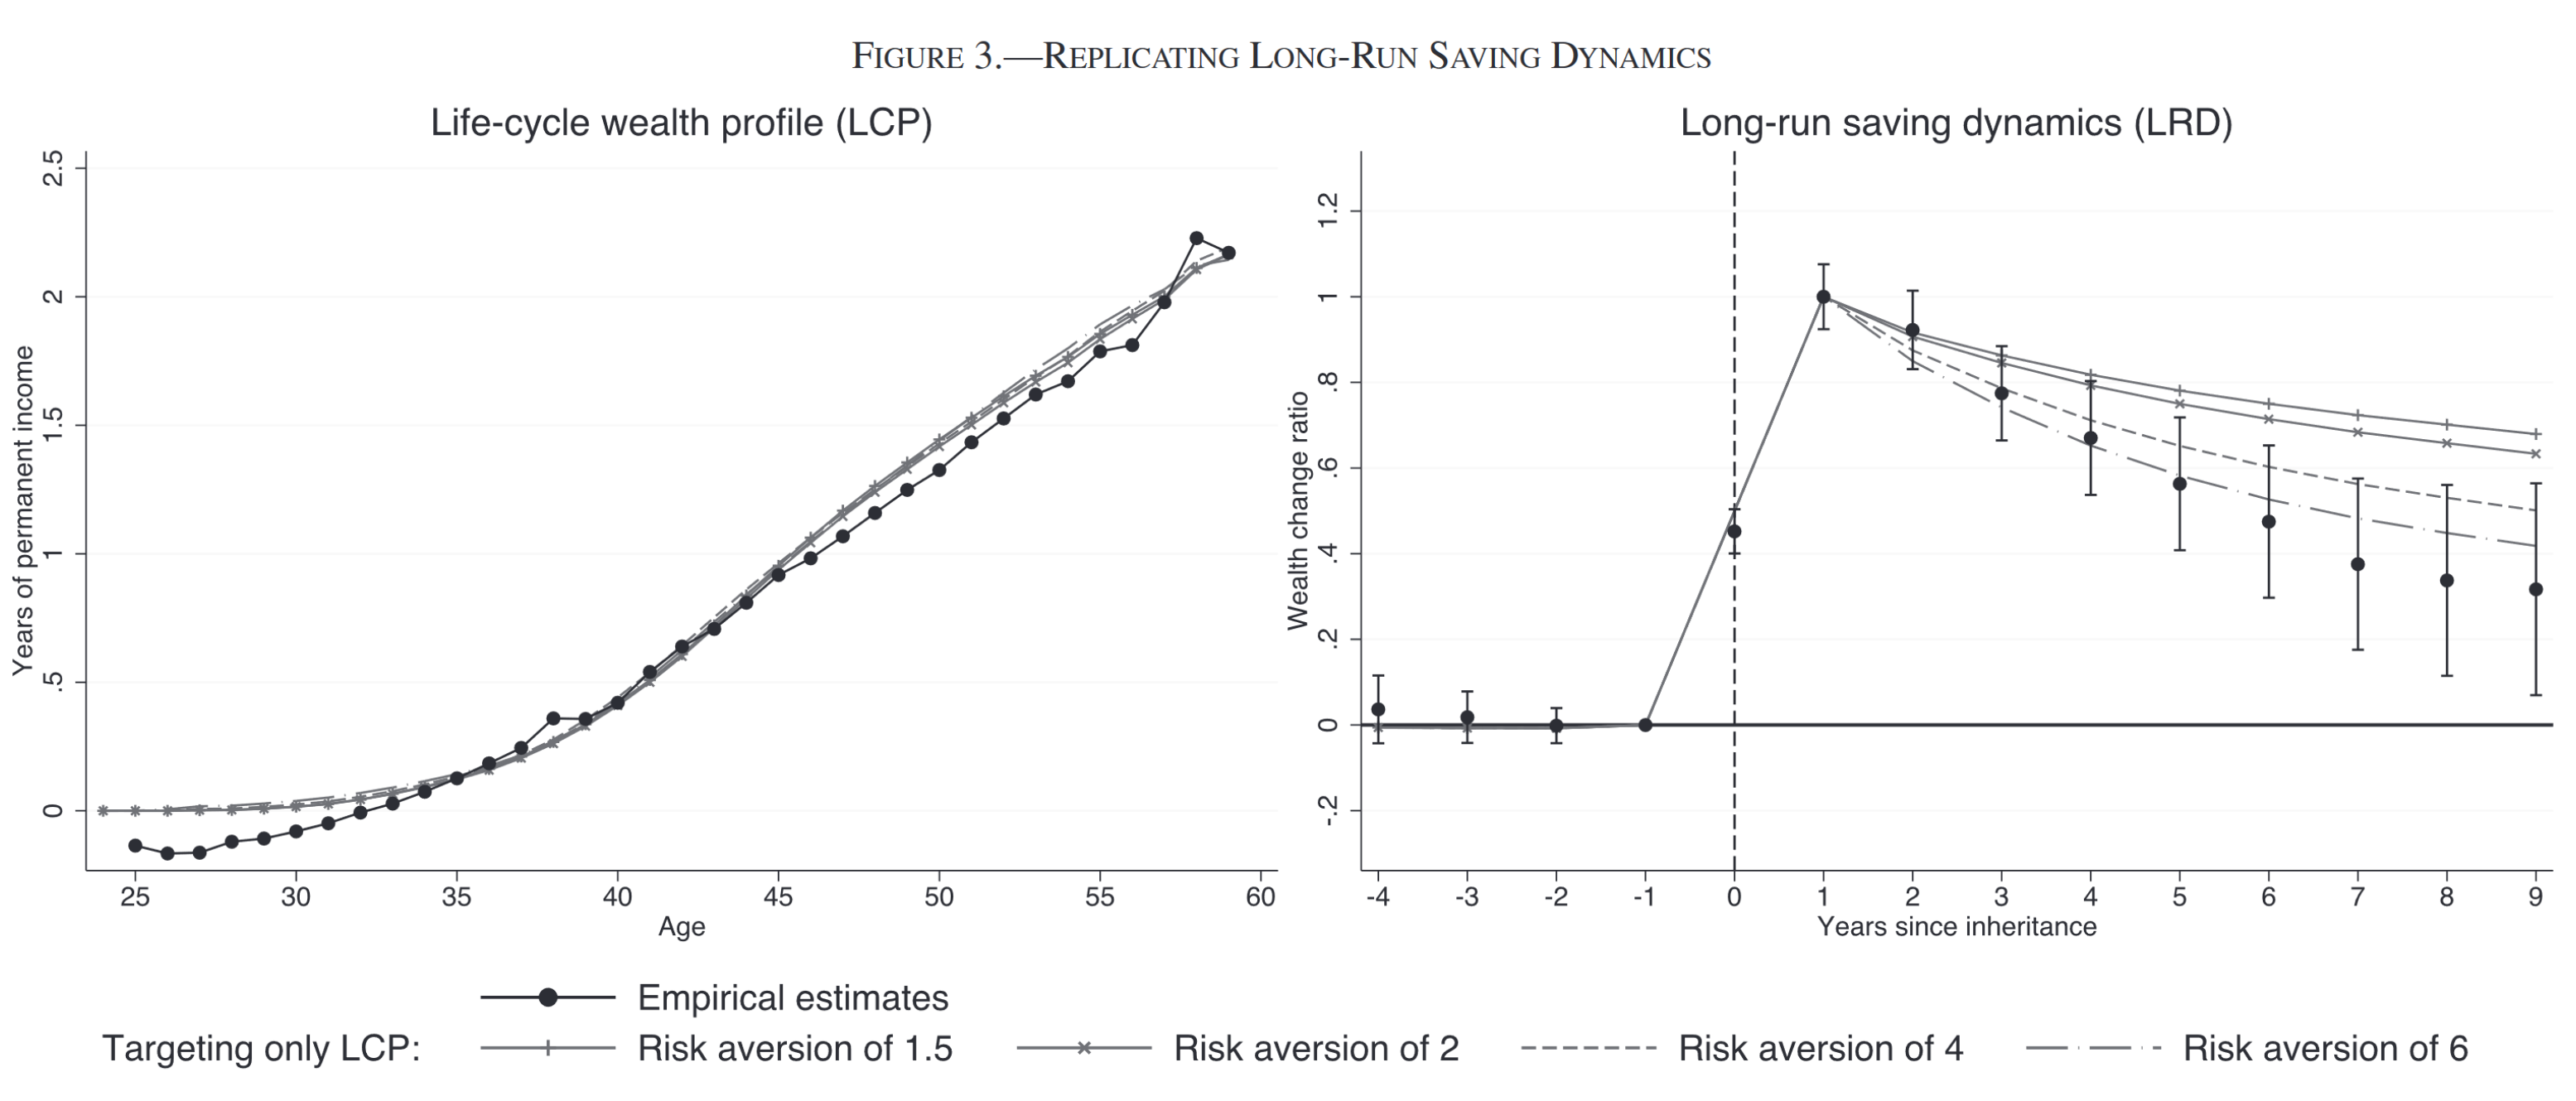
\includegraphics[width=0.95\textwidth]{figs/Druedahl_Martinello}\textbackslash{}

Source: Druedahl and Martinello (2022)
\end{frame}

\begin{frame}{2. More realistic income risk (I)}
\protect\phantomsection\label{more-realistic-income-risk-i}
Annual earnings-changes are far from log-normal:

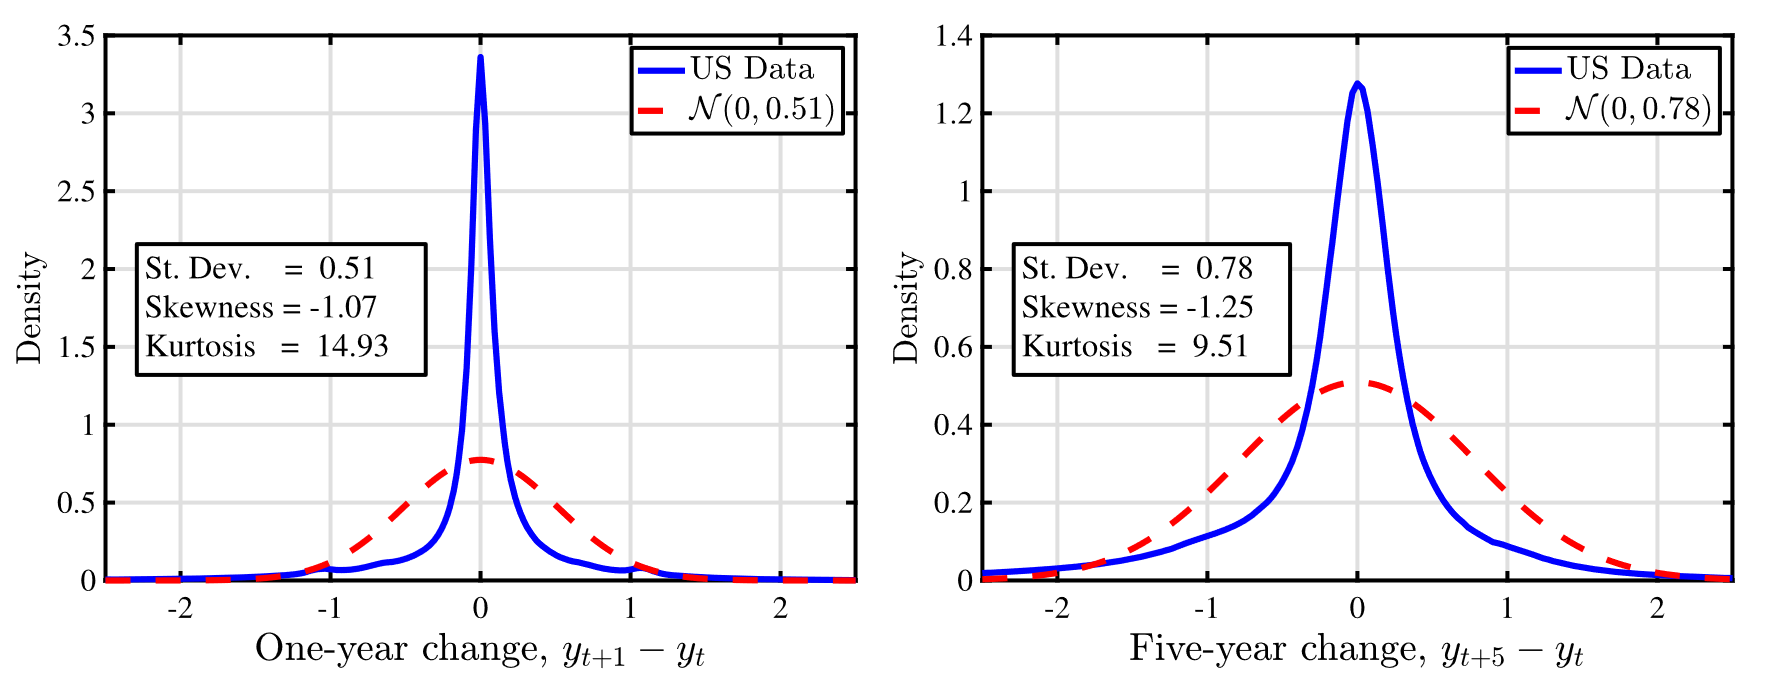
\includegraphics[width=1\textwidth]{figs/Guvenen}

Source: Guvenen et al.~(2021)
\end{frame}

\begin{frame}{2. More realistic income risk (II)}
\protect\phantomsection\label{more-realistic-income-risk-ii}
Many with zero-growth month-month:

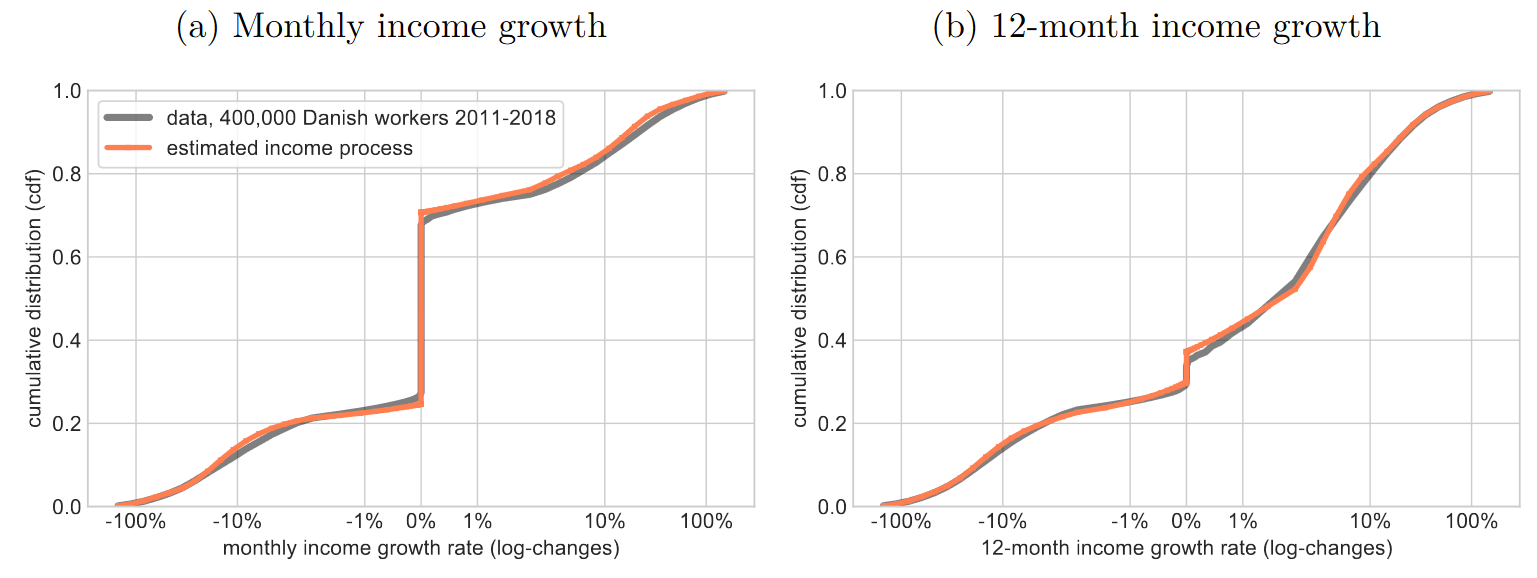
\includegraphics[width=1\textwidth]{figs/HighFreqIncDyn}

Source: Druedahl et al.~(2021)
\end{frame}

\begin{frame}{3. Epstein-Zin}
\protect\phantomsection\label{epstein-zin}
\vspace{-6mm}

\[
\begin{aligned}
v_{t}\left(z_{t},m_{t}\right) & = & \max_{c_{t}}\left[\left(1-\beta\right)\cdot c^{1-\sigma}_{t}+\beta\cdot w^{1-\sigma}_{t+1}\right]^{\frac{1}{1-\sigma}}\\
& \text{s.t.} & \,\,\,w_{t+1}\equiv\mathbb{E}_{t}\left[v_{t+1}\left(z_{t+1},m_{t+1}\right)^{1-\gamma}\right]^{\frac{1}{1-\gamma}}\\
&  & \,\,\,m_{t+1}=(1+r)(m_{t}-c_{t})+y_{t+1}
\end{aligned}
\]

\begin{itemize}
\item
  \vspace{-4mm}

  \textbf{Preferences:}

  \begin{enumerate}
  \tightlist
  \item
    Patience: \(\beta\)
  \item
    Intertemporal substitution: \(\sigma\)
  \item
    Risk-aversion: \(\gamma\)
  \end{enumerate}
\item
  \textbf{Euler-equation:}
  \(c^{-\sigma}_{t}=\beta R\cdot\mathbb{E}_{t}\left[c^{-\sigma}_{t+1}\cdot\left(\frac{w_{t+1}}{v_{t+1}}\right)^{\gamma-\sigma}\right]\)\vspace{2mm}

  \begin{enumerate}
  \tightlist
  \item
    FOC:
    \(0=v^{\sigma}_{t}\cdot\left[\left(1-\beta\right)\cdot c^{-\sigma}_{t}-\beta R\cdot w^{\gamma-\sigma}_{t+1}\cdot\mathbb{E}_{t}\left[v^{-\gamma}_{t+1}\cdot\frac{\partial v_{t+1}}{\partial m_{t+1}}\right]\right]\)\vspace{1mm}
  \item
    Envelope condition:
    \(\frac{\partial v_{t}\left(z_{t},m_{t}\right)}{\partial m_{t}}=v^{\sigma}_{t}\cdot\left(1-\beta\right)\cdot c^{-\sigma}_{t}\)
  \end{enumerate}
\end{itemize}
\end{frame}

\begin{frame}{4. Deep learning}
\protect\phantomsection\label{deep-learning}
\begin{itemize}
\item
  \textbf{Curse of dimensionality:}

  \begin{enumerate}
  \tightlist
  \item
    Many states
  \item
    Many choices
  \item
    Many shocks
  \end{enumerate}
\item
  \textbf{Deep (reinforcement) learning:}

  \begin{enumerate}
  \tightlist
  \item
    Approximate value and policy functions with \emph{neural networks}
  \item
    Approximate on simulation sample rather than on grid
  \item
    Automatic differentiation (backpropagation) and GPUs for speed
  \end{enumerate}
\item
  \textbf{Examples:} Maliar and Maliar (2021) and Azinovic and
  Scheidegger (2022)
\item
  \textbf{Working paper:} Druedahl and Røpke (2025)

  Python package:
  \href{https://github.com/NumEconCopenhagen/EconDLSolvers}{EconDLSolvers}
\end{itemize}
\end{frame}

\end{document}
